\chapter{Characterisation of the calorimeter time resolution}
\label{ch:Cobalt_study}

The precise knowledge of the different particle interaction times in the optical modules of the SuperNEMO calorimeter is important to better understand and reject the background.
For example, the study of electron time-of-flight allows us to distinguish internal events (occurring within the source foils) from external events (radioactive decays occurring outside the source foils, for example in the PMTs or in the iron shielding).

During the commissioning phase, a lot of work, presented in the next chapter, was achieved to calibrate the detector.
Following on from this task and completing it, a great part of my PhD was allocated to determine the time resolution of the SuperNEMO calorimeter, and to provide tools to the collaboration to purchase this analysis.

In this chapter we present different studies conducted in order to characterise the time response of the SuperNEMO optical modules.
Although the goal of the presented studies is to characterise the time resolution of the SuperNEMO calorimeter, some detector adjustments were still ongoing at the time of the acquisition, that could influence the presented results.
Especially, the energy calibration described in Sec.~\ref{sec:comm_energy_calibration} was not complete, and the Light Injection System presented in Sec.~\ref{sec:LIS} was not yet fully operational.
However, all the work presented here is necessary in the framework of the first calorimeter calibration.
Moreover, I provide all the analysis tools for the collaboration, with a view to doing a possible update, once the whole demonstrator calibration will be achieved.

The first study presented in this chapter focuses on the characterisation of the time resolution of the SuperNEMO calorimeter, using a calibration source made of Cobalt $60$.
In the second part of this chapter, we study the possibility to gather informations on the calorimeter time resolution using the Light Injection System, a set-up initially designed to calibrate in energy the calorimeter.

%%%%%%%%%%%%%%%%%%%%%%%%%%%%%%%%%%%%%%%%%%%%%%%%%%%%%%%%%%%%%%%%%%%%%%%%%%%%%%%%%%%%%%%%%%%%%%%%%%%%%%%%%%%%%%%%%%%%%%%%%%%%%%%%
\section{Interaction of particles in the SuperNEMO scintillators}
\label{sec:scintillator_interactions}

Understanding how particles interact in the SuperNEMO scintillators is essential.
The calorimeter part of the demonstrator mainly aims to detect electrons and photons.
In this section, we review ***.


\subsection{Interaction of electrons}

Electrons interact with matter through one of two processes: elastic scattering on a nucleus, or inelastic scattering on an atomic electron.
Inelastic scatterings are dominant for polystyrene scintillators and occur through two different forms: coherent scattering with the electron cloud, and radiative energy losses (the so-called bremsstrahlung effect).
In Fig.~\ref{subfig:electron_attenuation} is displayed the stopping power of electrons in polystyrene for these two processes.
\begin{figure}[h]
  \centering
  \begin{subfigure}[t]{0.48\textwidth}
    \centering
    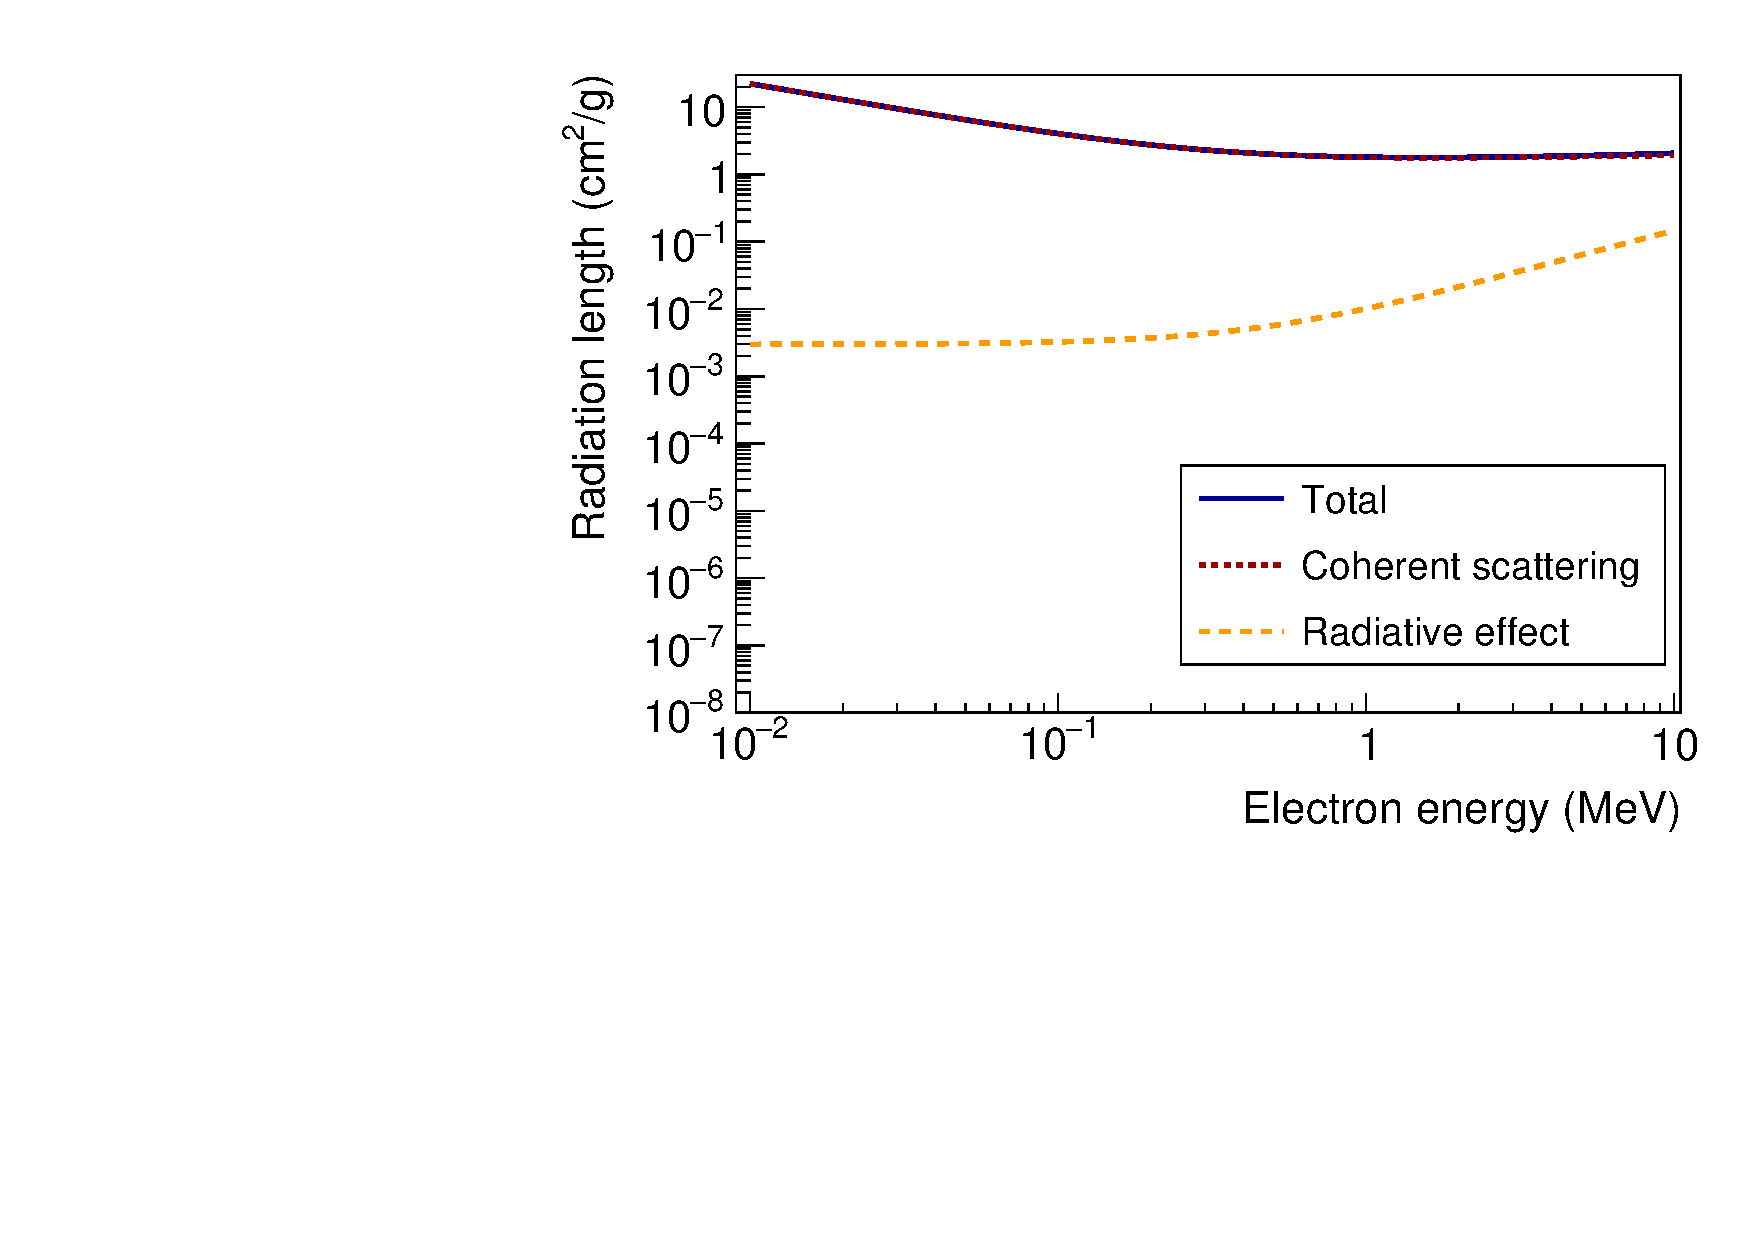
\includegraphics[width=1\textwidth]{commissioning/fig_commissioning/electron_energy_loss.pdf}
    \captionsetup{justification=centering}
    \caption{
      \label{subfig:electron_attenuation}}
  \end{subfigure}
  \hfill
  \begin{subfigure}[t]{0.48\textwidth}
    \centering
    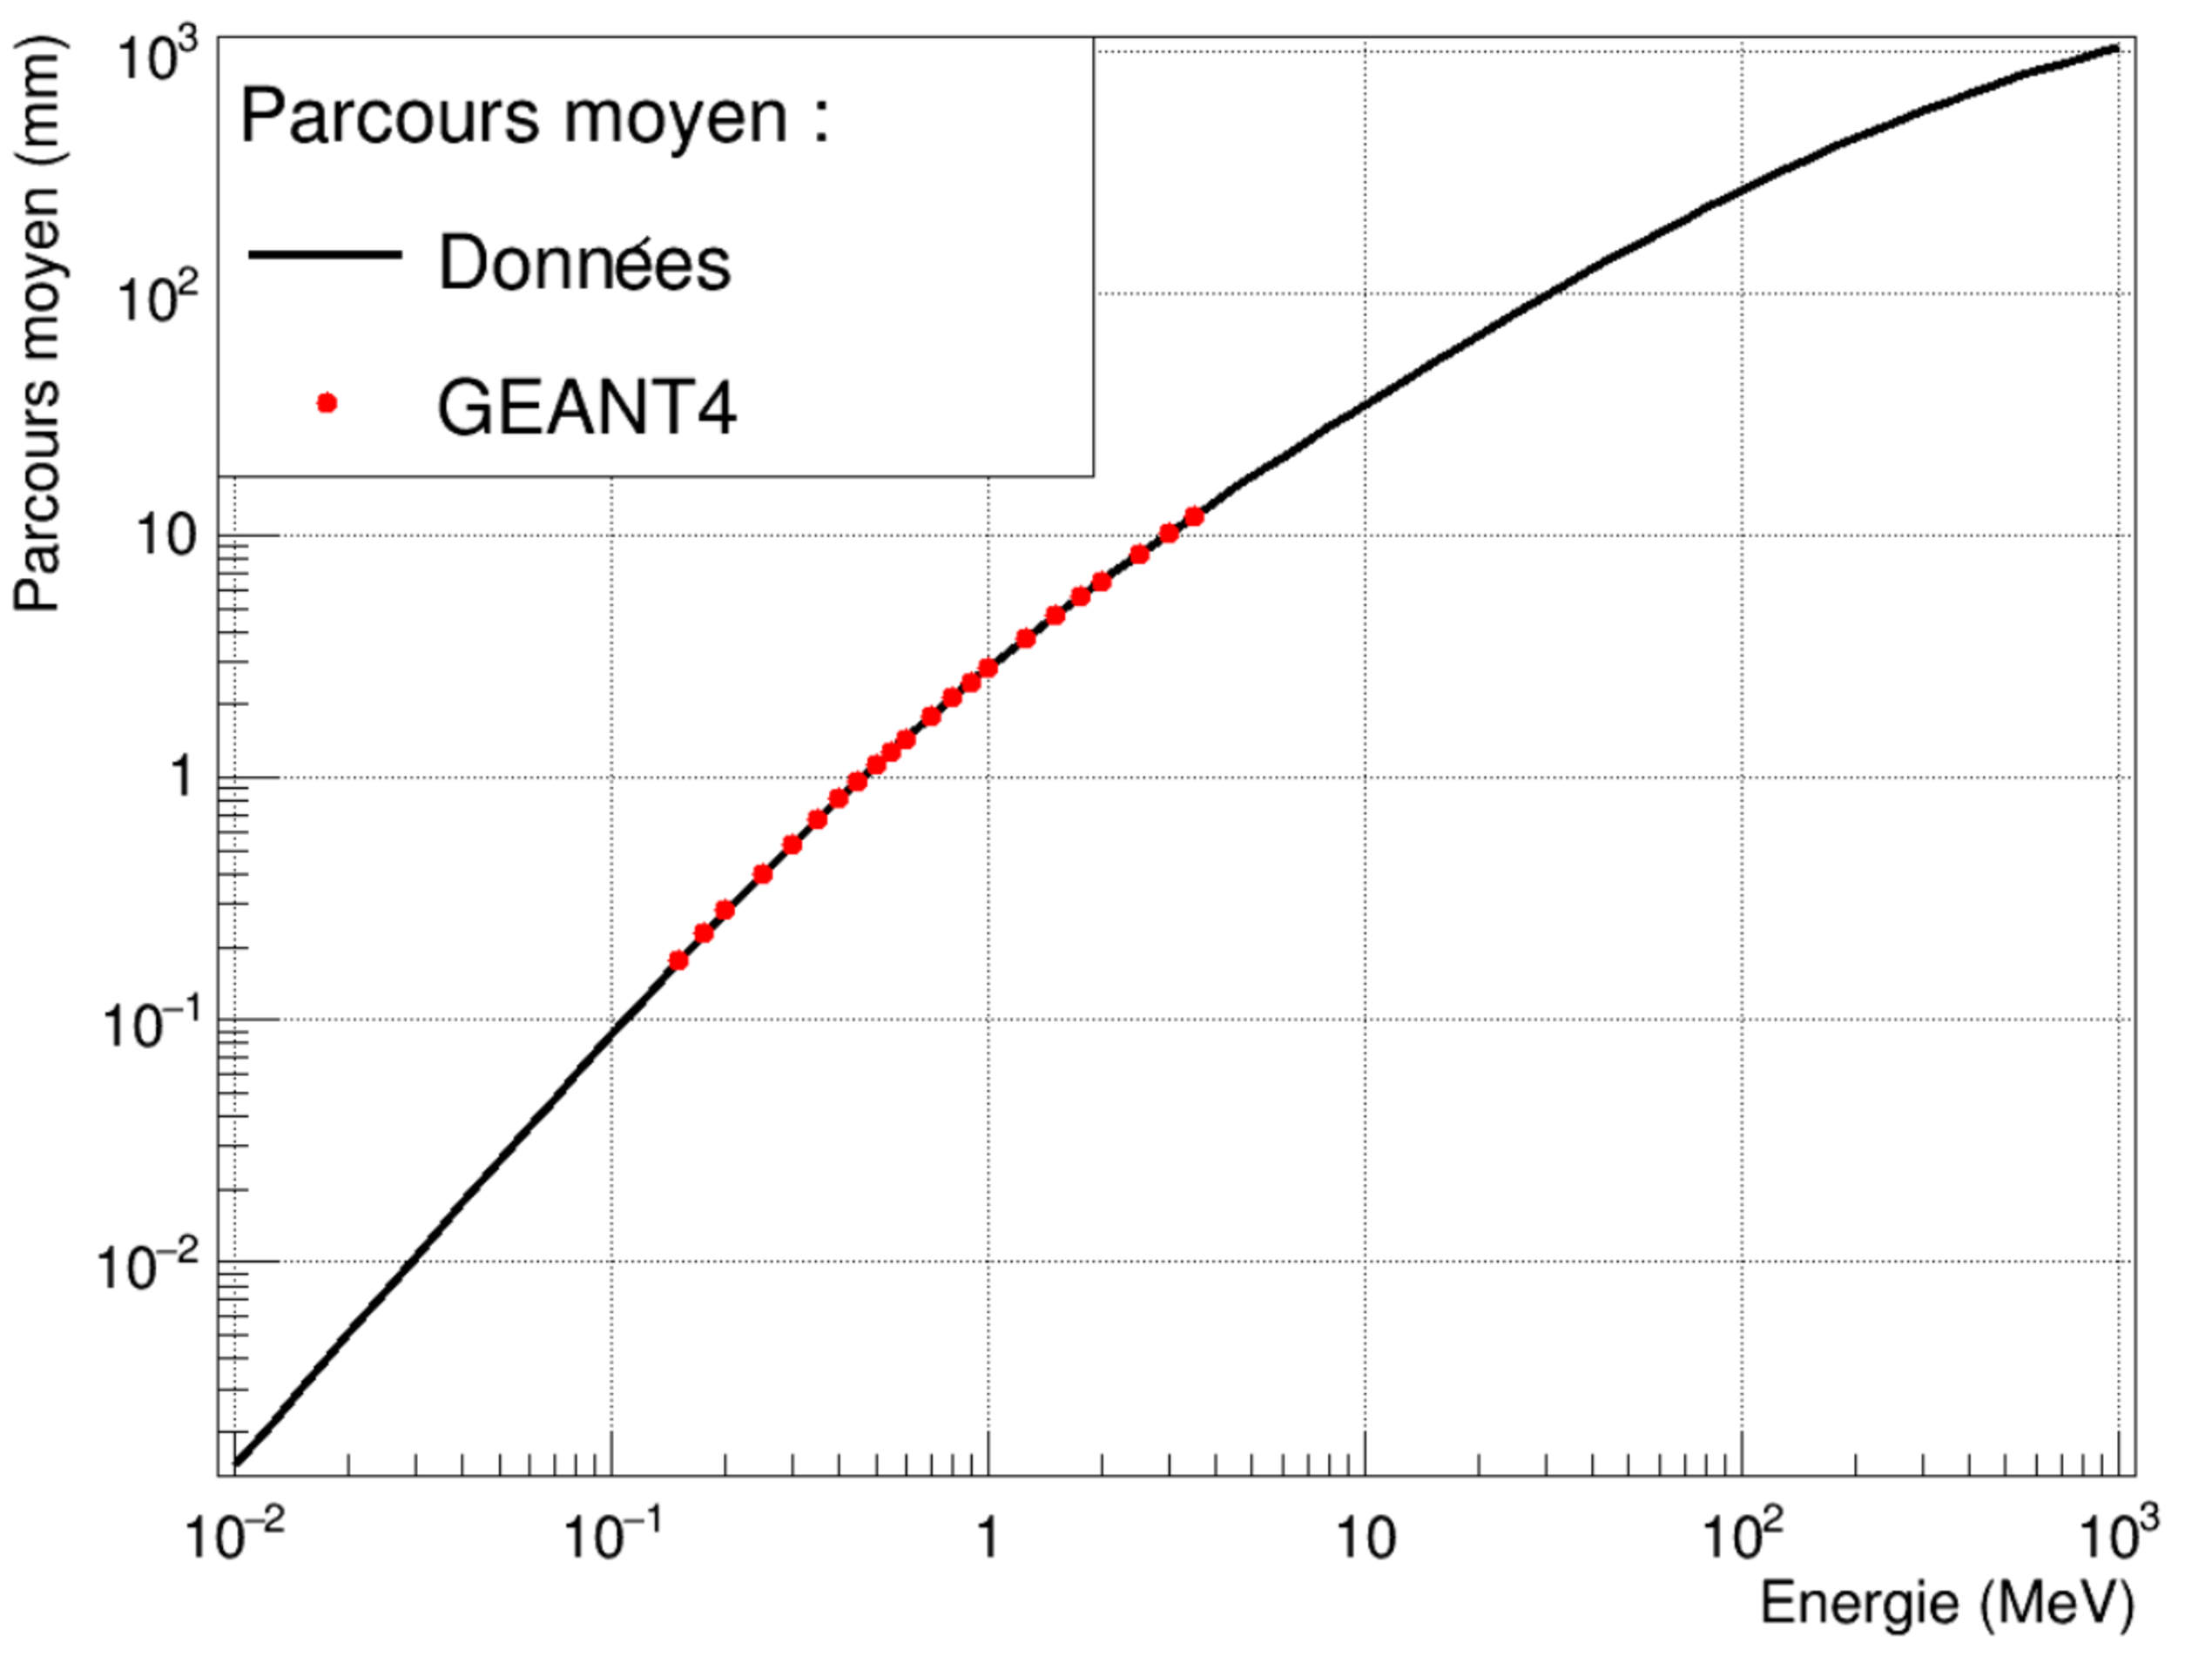
\includegraphics[width=1\textwidth]{commissioning/fig_commissioning/free_path_electrons.pdf}
    \captionsetup{justification=centering}
    \caption{\label{subfig:electron_free_path}}
  \end{subfigure}
  \caption{Stopping power (a) and mean free path (b) for electrons in polystyrene.
    (a) Energy losses through radiative effect (orange dashed line) and coherent scattering (red dashed line), which is the dominant process for the considered energy range~\cite{web:nist_estar}.
    %  operate mainly through coherent scattering.
    (b) At $1$ MeV, the mean free path of an electron is about $3$ mm.
    Adapted from~\cite{HuberThesis}.
  }
\end{figure}
Electrons detected in the SuperNEMO calorimeter should deposit a minimal energy of $50$ keV (the acquisition low energy threshold) and a maximal energy of few MeV (depending on the $\twonu$ isotope).
In this energy range, collisions with the electron cloud are preponderant compared with radiative energy losses.
In Fig.~\ref{subfig:electron_free_path}, we give informations about the mean free path of an electron in polystyrene.
In particular, we observe that an electron of $1$ MeV penetrates, in average, several millimetres into a polystyrene scintillator.


\subsection{Interaction of photons}

Photons travelling in  matter can interact with the electronic cloud, through three main processes, whose contributions are presented in fig.~\ref{subfig:photon_energy_loss}, depending on their energies.
\begin{figure}[h]
  \centering
  \begin{subfigure}[t]{0.48\textwidth}
    \centering
    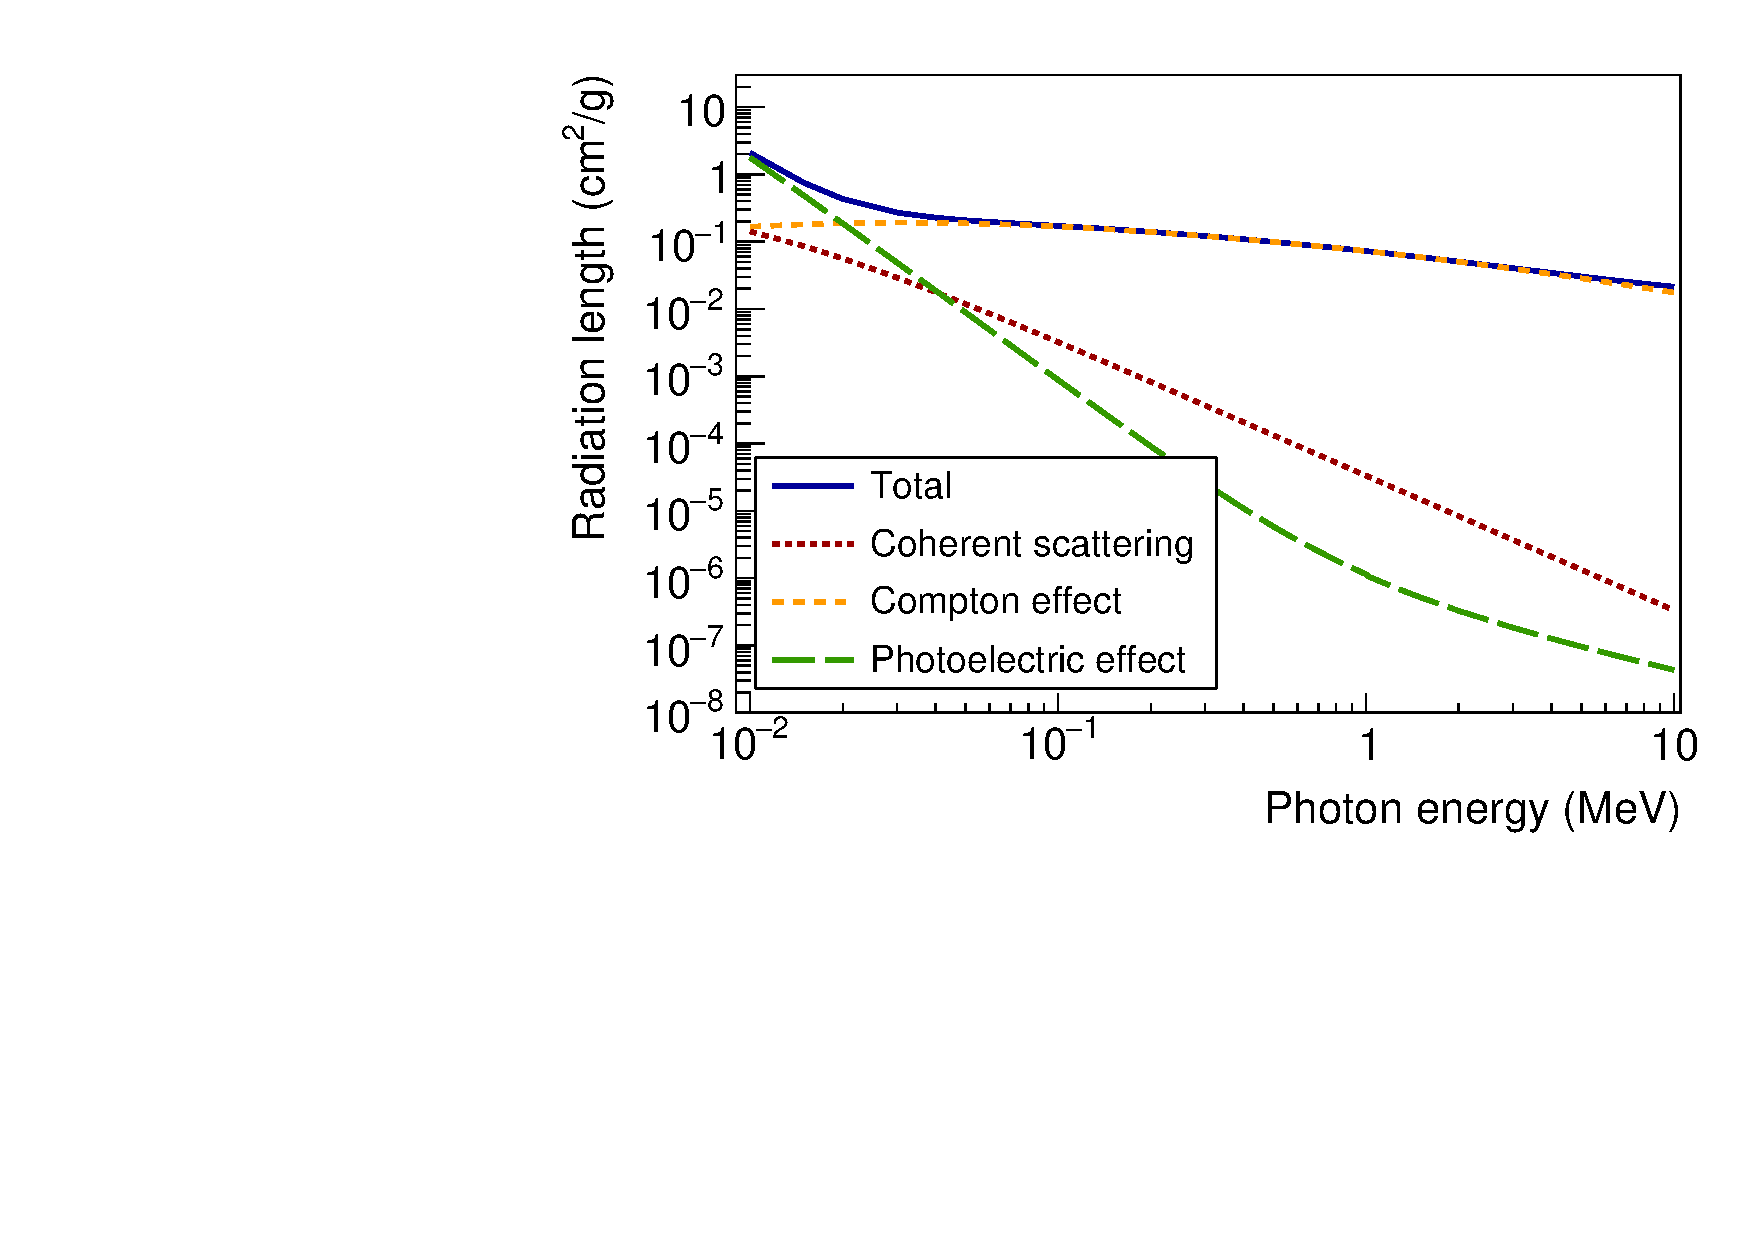
\includegraphics[width=1\textwidth]{commissioning/fig_commissioning/photon_energy_loss.pdf}
    \captionsetup{justification=centering}
    \caption{\label{subfig:photon_energy_loss}}
  \end{subfigure}
  \hfill
  \begin{subfigure}[t]{0.48\textwidth}
    \centering
    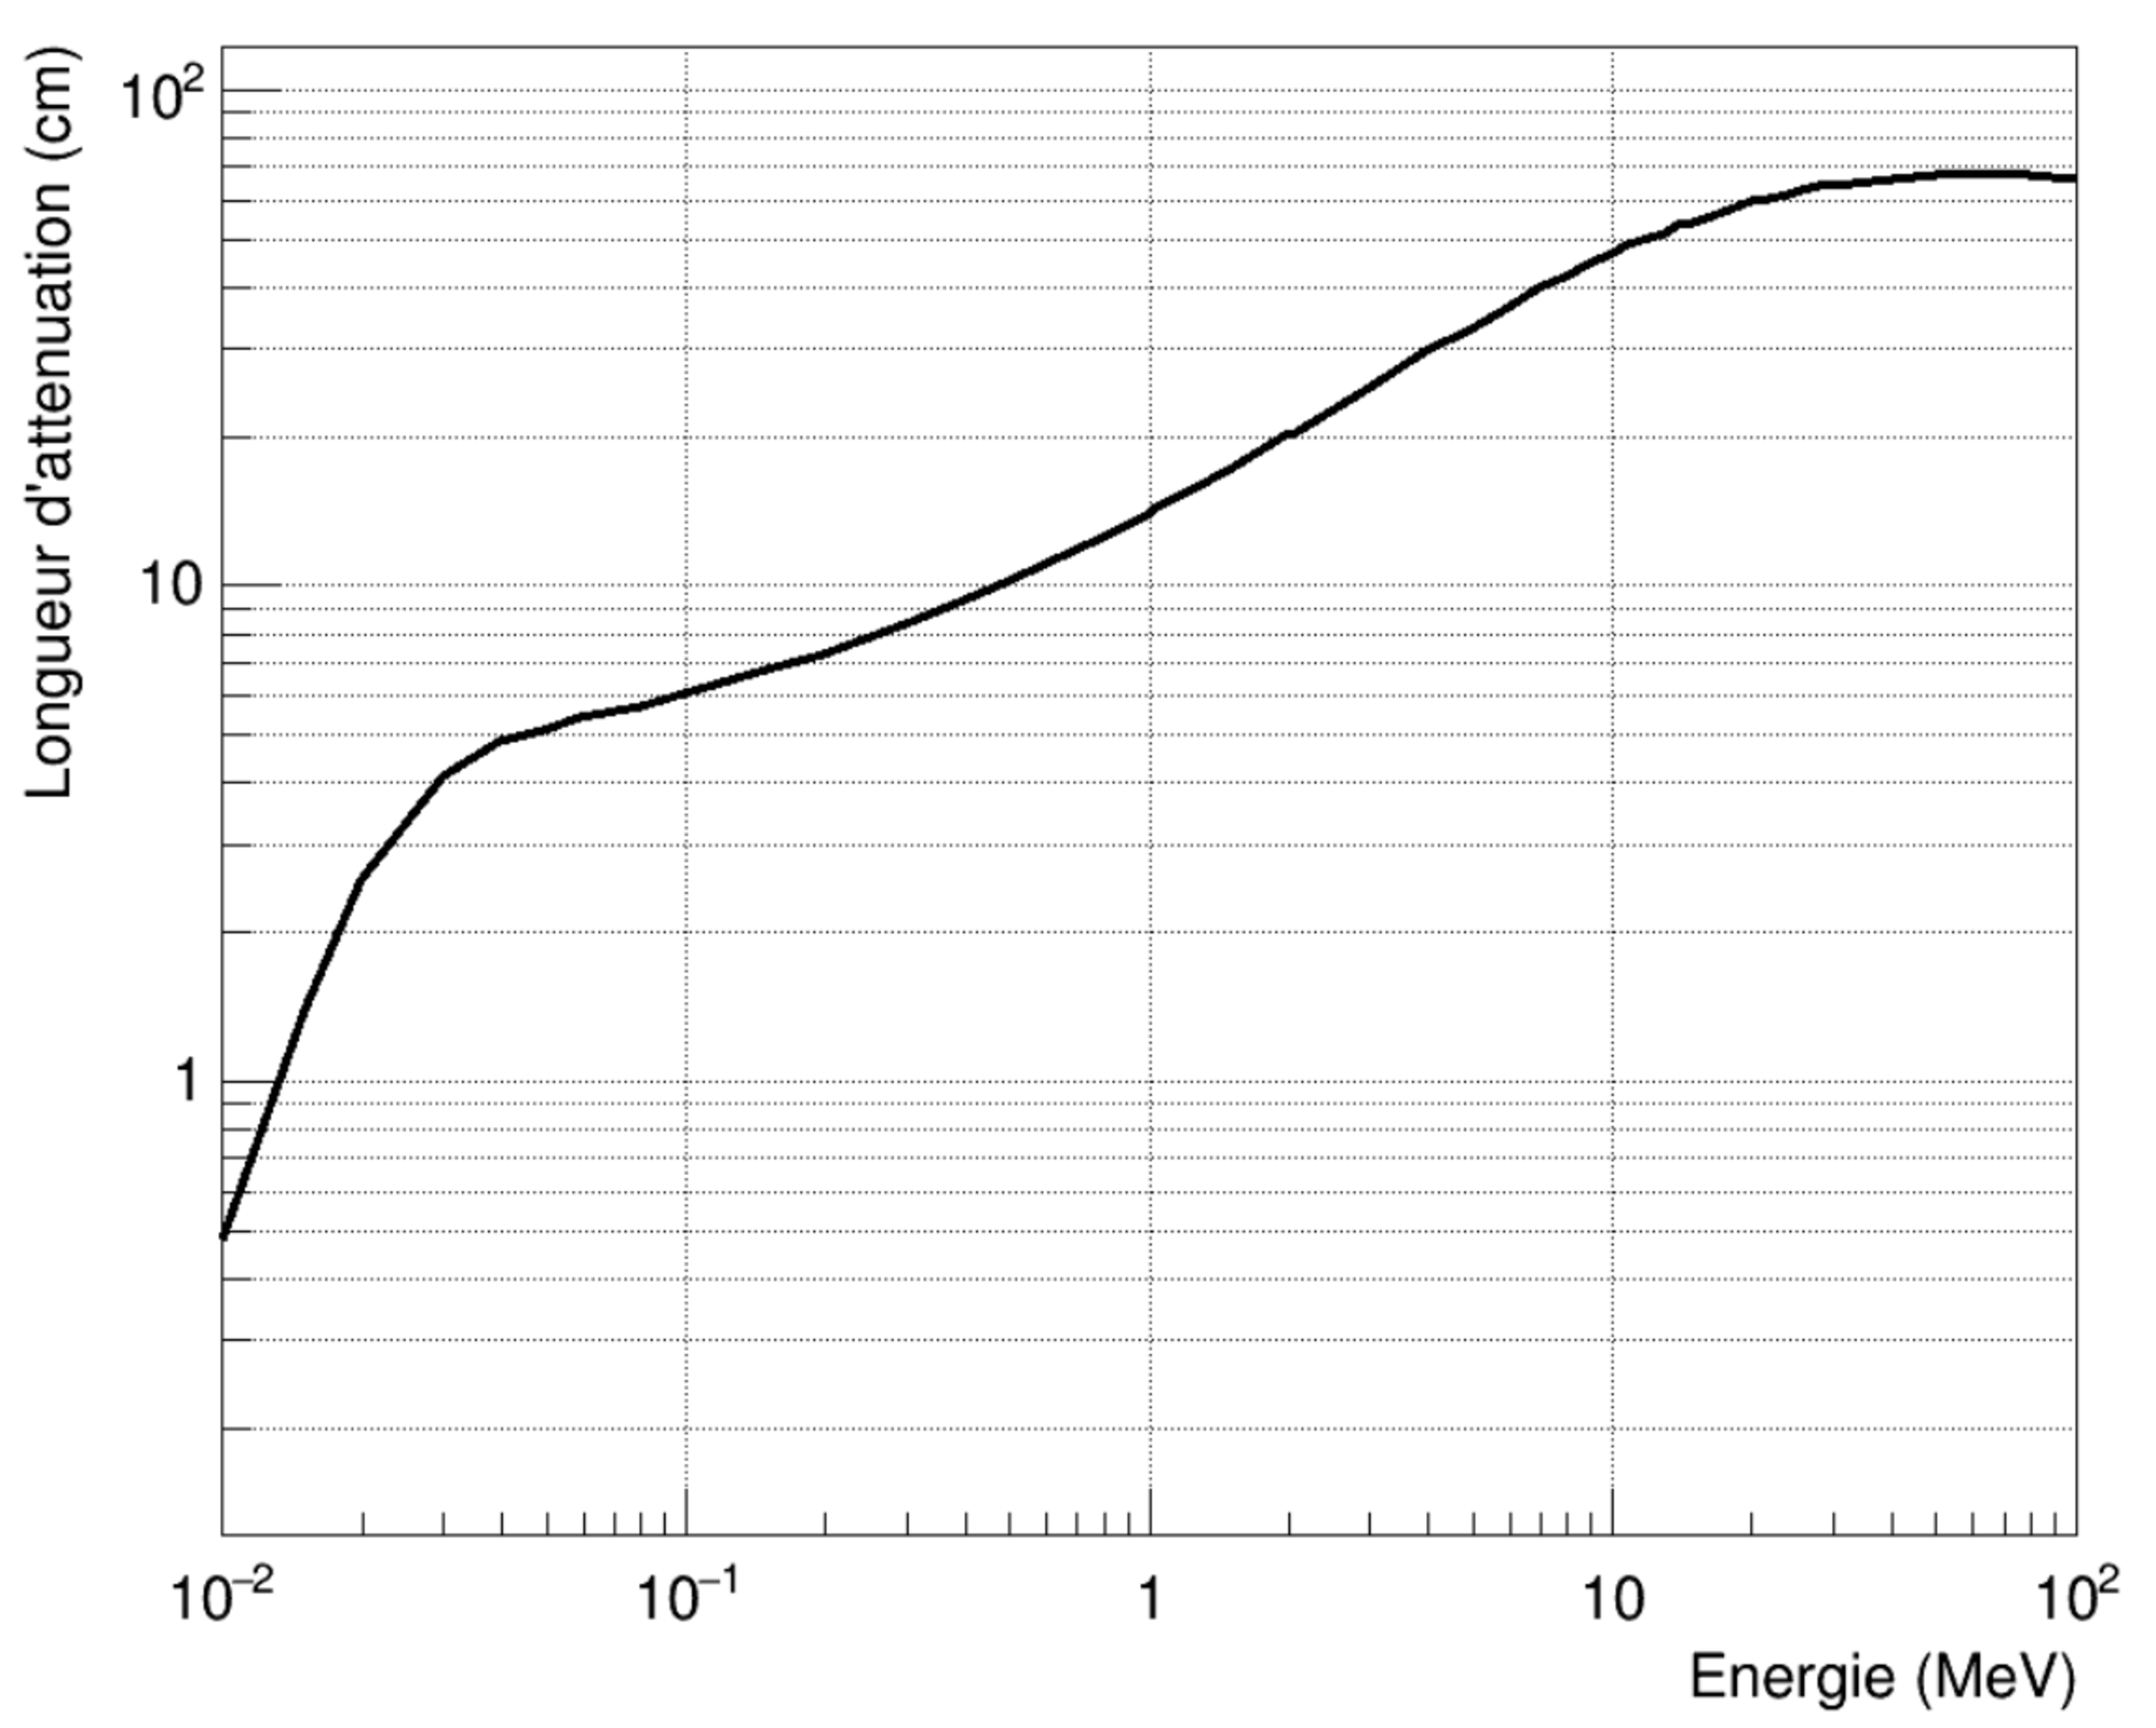
\includegraphics[width=1\textwidth]{commissioning/fig_commissioning/attenuation_length_photons.pdf}
    \captionsetup{justification=centering}
    \caption{\label{subfig:attenuation_length_photons}}
  \end{subfigure}
  \caption{Linear attenuation coefficient (a) and attenuation length (b) for $\gamma$ radiations in a plastic scintillator made of polystyrene.
    (a) In the considered energy range of $10$ keV $ -\; 10$ MeV, $\gamma$ radiations interact with matter mainly through Compton diffusion~\cite{web:nist_Xcom}.
    (b) The attenuation length of a $\gamma$ radiation is about $10$ cm at $1$ MeV.
    Adapted from~\cite{HuberThesis}.
  }
\end{figure}
Low-energy photons mainly interact with the electron cloud, either through photoelectric effect ($\gamma$ radiation is fully absorbed by an electron of the cloud), or through coherent (so-called Rayleigh) scattering.
But the dominant effect, for energies between $10$ keV and $10$ MeV, is the Compton inelastic scattering of a $\gamma$ with an atomic electron.
In Fig.~\ref{subfig:attenuation_length_photons}, we display the mean attenuation length of a $\gamma$ radiation in polystyrene scintillators, with energy.
Thus, most of $1$ MeV $\gamma$ radiations will interact around $10$ cm inside the scintillating material.

At the considered energy range ($10$ keV $ -\; 10$ MeV), the interaction of photons with matter is dominated by Compton effect, while the electrons interact mainly through coherent scattering.
The SuperNEMO scintillators are designed to detect such particles.
Photons have a high probability to interact inside the volume of the scintillator, while electrons are stopped in the first few millimetres.

The following section are devoted to the study of the time resolution of the SuperNEMO optical modules.



%%%%%%%%%%%%%%%%%%%%%%%%%%%%%%%%%%%%%%%%%%%%%%%%%%%%%%%%%%%%%%%%%%%%%%%%%%%%%%%%%%%%%%%%%%%%%%%%%%%%%%%%%%%%%%%%%%%%%%%%%%%%%%%%
\section{Measurement of the time resolution with a $^{60}$Co source}
\label{sec:Co_analysis}
This section is dedicated to detail the time resolution study performed using a Cobalt $60$ source, exploiting the time characteristic of two photons emitted during the radioactive disintegration process of this nucleus.
A great proportion of the whole SuperNEMO demonstrator was successfully characterised using this radioactive source.

\subsection{Description of Cobalt $60$ nucleus}
\label{subsec:CoSource}
The Cobalt $60$ is a man-made isotope, with a $5.27$ years half-life, of which we provide the main interesting properties in the simplified decay scheme of Fig.~\ref{fig:Co_decay_scheme}.
\begin{figure}[h]
  \centering
  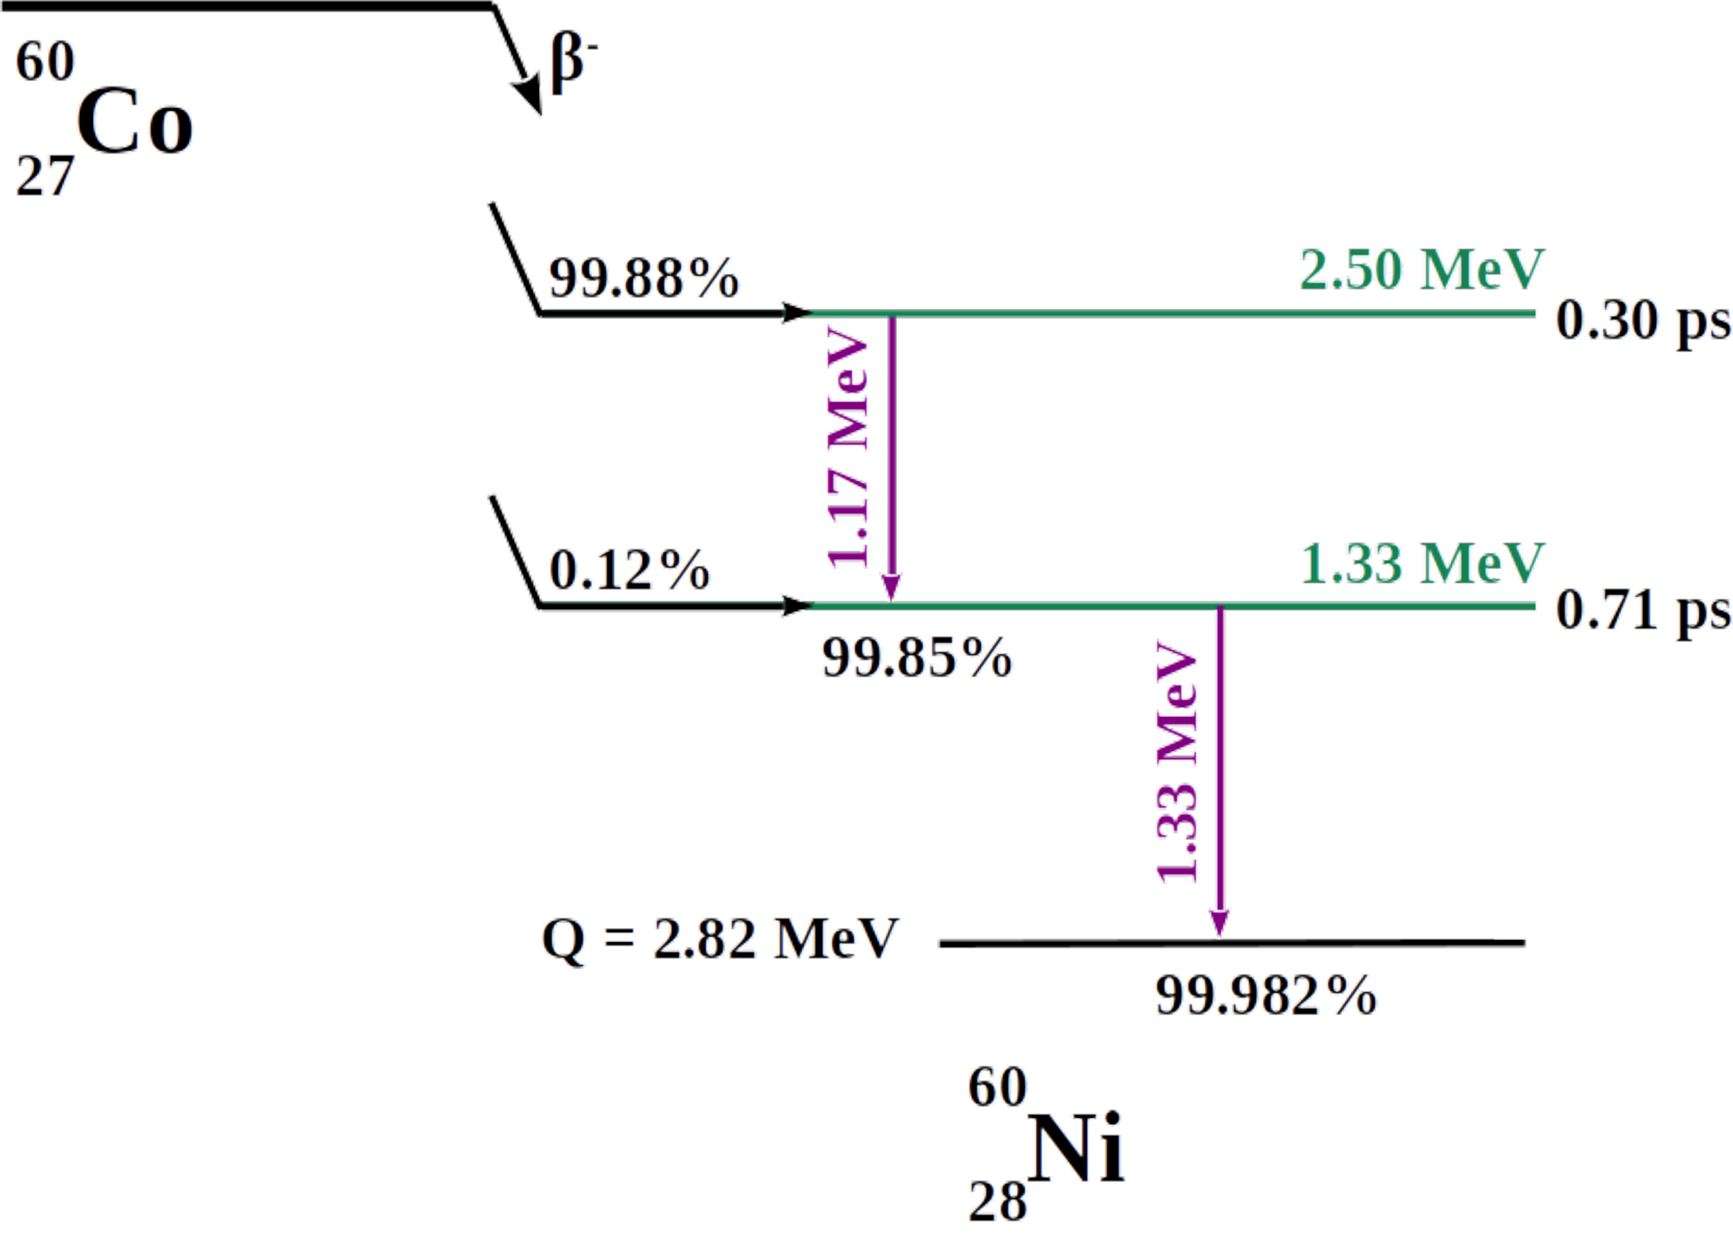
\includegraphics[width=9cm]{commissioning/fig_commissioning/Co_decay_scheme.pdf}
  \caption{A simplified decay scheme for Cobalt $60$ \cite{web:nucleide}.
    The Cobalt decays, through $\beta^{-}$, predominantly to the $2.50$ MeV state.
    Then, two succesive $\gamma$'s (whose energy levels are represented in green) are emitted in $99.83$\% of the cases.
    The two photons have an energy of $1.17$ MeV and $1.33$ MeV, respectively.
    As the life-time of the $1.33$ MeV energy level is short ($<1$ ps) with respect to the timing precision of the calorimeter, the two photons can be considered as emitted in coincidence.
    We use this property to calibrate in time the demonstrator optical modules.
    \label{fig:Co_decay_scheme}}
\end{figure}
This unstable nucleus spontaneously decays, through the $\beta^{-}$ process, into an excited state of Nickel $60$.
To reach the ground state of the Nickel $60$, the nucleus goes through two successive energy levels, emitting in $99.83$\% of the cases two photons of $1.17$ MeV and $1.33$ MeV, respectively.
The life-time of the second energy level is under the picosecond, thus very short with respect to the expected timing precision of the calorimeter.
Therefore, the two photons are considered as emitted in coincidence.

We aim to exploit these two photons emitted after the $\beta^{-}$ disintegration to determine the calorimeter time resolution.

\subsection{Time response of optical modules}
\label{subsec:OMtimeResponse}

In order to characterise the energy and time-of-flight of incoming particles (photons, electrons), each calorimeter block of SuperNEMO is composed of a scintillator and a photomultiplier.
As detailed in Chapter~\ref{ch:detector}, the purpose of the scintillator material is to stop the incoming particles, which will induce the production of the so-called optical photons.
The optical photons reaching the photomultiplier photocathode are then converted into electrons, with an efficiency called quantum efficiency.
After amplification, electrons are collected by the anode which delivers an electric signal whose charge proportional to the initial amount of incident photoelectrons.
This signal is then transmitted, via the PM voltage divider, to the electronic readout, where the signal is sampled.
The particle energy, as well as the time-of-flight, can be extracted from the signal waveform analysis.
Each step of the particle detection process, from the incident particle interaction inside the scintillator, to the signal sampling at the electronic readout, can have an impact on the precise time measurement of the charged particle.
In Chapter~\ref{ch:detector} and \ref{ch:timediff} we introduced the so-called calorimeter time resolution $\sigma_t$, which encapsulates the global uncertainty on the time-of-flight measurement of particles into the calorimeter (Eq.~\eqref{eq:sigma_t}).
The squared time-resolution can therefore be expressed as the sum of two contributions:
the scintillator resolution $\sigma_{t, \textrm{sc}}^{2}$, and the PMT resolution $\sigma_{t, \textrm{PM}}^{2}$,
\begin{equation}
  \sigma_{t}^{2}=\sigma_{t,\text{sc}}^{2}+\sigma_{t,\text{PM}}^{2}\,.
  \label{eq:Co_sigma_t}
\end{equation}
In the following, we detail in depth the physical origins of these terms.

\subsubsection*{Scintillator time dispersion}
The scintillator temporal dispersion $\sigma_{t,\text{sc}}$ in Eq.~\eqref{eq:Co_sigma_t} receives contributions mainly from two important characteristics of the scintillator operating principle.

\paragraph{Interaction point:}
The incoming particle's interaction point location inside the scintillator block highly contributes to the scintillator temporal uncertainty, and depends on the incident particle type.
In fact, this effect will not have the same impact on time dispersion, depending on whether the incident particle is a photon or an electron.
In Fig~\ref{fig:photon_scintilator} are schemed the interactions of a photon and that of an electron for the specific case of a SuperNEMO plastic scintillator.
\begin{figure}[h]
  \centering
  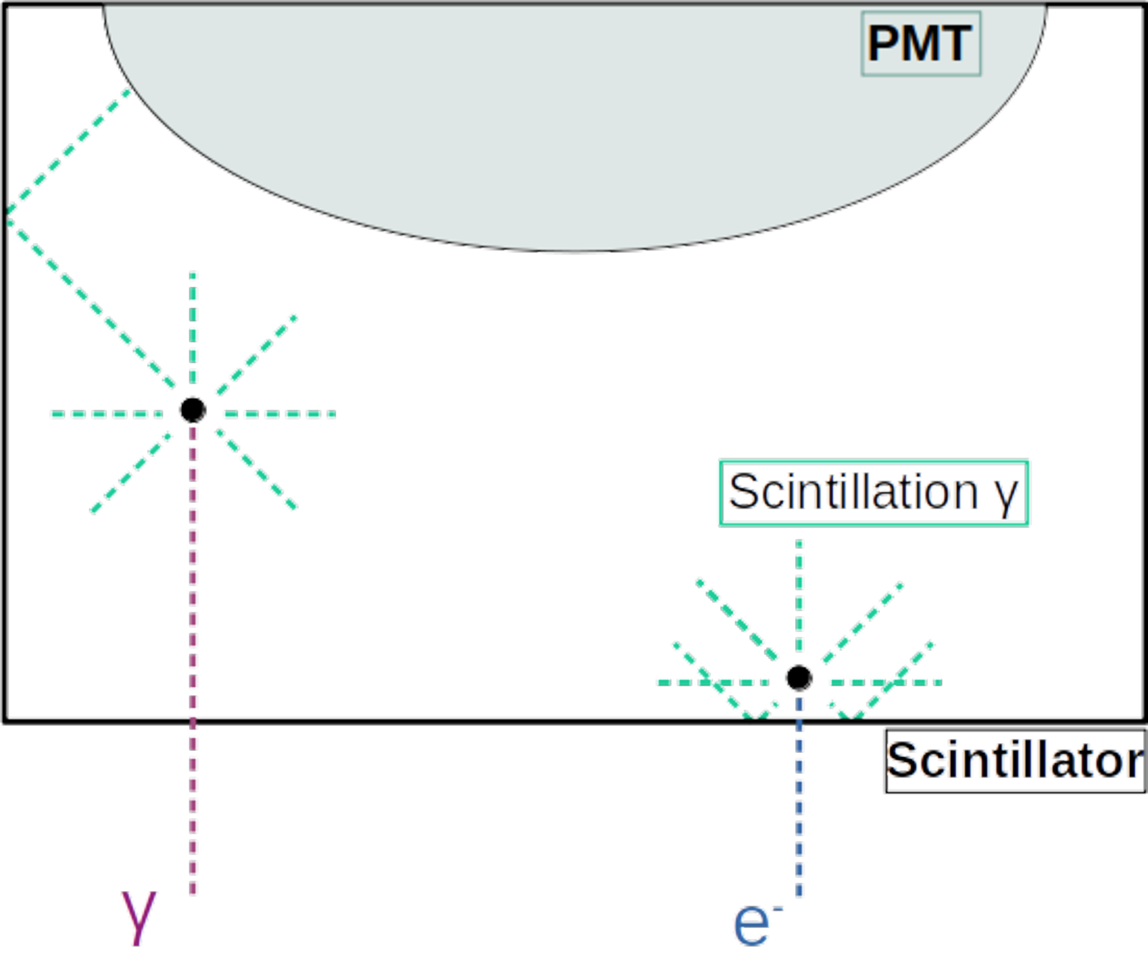
\includegraphics[width=8cm]{commissioning/fig_commissioning/Co_multi_reflection.pdf}
  \caption{A scheme of interaction of particles in a scintillator.
    The photon case is displayed on the left in pink dotted line, and the electron case is on the right in dark blue dotted line.
    Both particles enter in the scintillator through the front face.
    Examples of interaction points inside the scintillator are represented by the black dots.
    The photons of scintillation emitted isotropically after the interaction are materialised by the bright green dotted lines.
    Due to different interaction probabilities in matter, the two particles intercat at different depths inside the scintillator.
    The photon can interact deeply inside the volume, while the electron has a high probability to stop within the first few millimetres.
    \label{fig:photon_scintilator}}
\end{figure}
In Sec.~\ref{sec:scintillator_interactions}, we exposed the different interaction types of photons and electrons.
We have also explained the origin of the differences that exist in terms of interaction depth between these two types of particles.
To remain consistent with these conclusions, we represent the electron as interacting in the first millimetres, while the photon stops deep inside the scintillator.
When a particle (photon or electron) interacts in the scintillating material, the absorbed energy leads to the isotropic emission of scintillation photons:
they propagate inside the scintillator, in all directions from the interaction point, at the speed of $c/n_{sc}$, with $n_{sc}$ the optical index of polystyrene, and $c$ the light speed in vacuum.
Depending on their initial direction, some of those photons propagate straight to the PMT (we name them the \emph{direct} photons), while others are at least reflected once on the scintillator surface, before reaching the PM glass.
This mechanism leads to time delays between direct and reflected photons.

In order to illustrate, and give an order of magnitude of this delay, let us consider an example where an incoming electromagnetic particle enters a scintillator from the front face, and interacts right in the centre of the scintillator volume.
After the scintillation emission process, a direct photon will reach the PM glass surface at time
\begin{equation}
  t_{s} = \frac{L}{2c/n_{sc}}\,,
\end{equation}
$L$ being the scintillator width.
Now, let us consider another photon, that we name \emph{backward reflected}, emitted in the opposite direction.
It will propagate, reflect on the front scintillator surface, and finally reach the PM at
\begin{equation}
  t_{r} = \frac{3L}{2c/n_{sc}}\,.
\end{equation}
This reflected photon is therefore delayed compared to the direct photon, with a time-shift of
\begin{equation}
  \Delta t^{r,s} = t_{r} - t_{s} = \frac{L}{c/n_{sc}}\,.
\end{equation}
In the case of a SuperNEMO scintillator, the length $L$ has been designed to $25$ cm, and the optical index is the one of polystyrene with $n_{sc}=1.5$.
Finally, for an incoming particle interacting at the centre of a SuperNEMO scintillator volume, a backward reflected scintillation photon will reach the PM glass $1.25$ ns later than a direct photon.
And this delay is even more important as the incident particle interacts deep inside the scintillator.

In view of the conclusions given in Sec.~\ref{sec:scintillator_interactions}, we know that photons have a higher probability of interacting far into the scintillator block, compared with electrons.
Therefore, this time-shift effect is all the more important for incoming photons, while it is quite negligible for incoming electrons, for which reflected photoelectrons reach the PM glass almost as the same time as the direct ones.

This mechanism increases the signal collection rising time at the PM anode, and boosts the scintillator time dispersion $\sigma_{t,\text{sc}}$, with $\sigma_{t,\text{sc}}^{\gamma}>\sigma_{t,\text{sc}}^{\text{e}^{-}}$.

\paragraph{Scintillating light emission:}
When a particle interacts in a SuperNEMO scintillator, two successive mechanisms of light absorption/re-emission take place.
Firstly, the excitation of scintillator molecules leads to the creation of fluorescence photons.
Afterwards, those optical photons are absorbed, then re-emitted by the POPOP agent, at higher wavelengths.
The characteristic times of these two processes contribute to increase the scintillator time dispersion $\sigma_{t,\text{sc}}$.
%% These two processes follow the same temporal distribution
%% \begin{equation}
%%   \mathcal{N}_{\text{photons}} = A\times e^{-t/\tau}\,,
%%   \label{eq:fluorescence_photons_time}
%% \end{equation}
%% with $\mathcal{N}_{\text{photons}}$ the number of generated photons at time $t$, $A$ a normalisation constant and $\tau$ the fluorescence characteristic time of the considered process.

Now that two main contributions accounting for the uncertainty on time measurement taken by the scintillator had been developed, we detail the origin of the second term of Eq.~\eqref{eq:Co_sigma_t}, $\sigma_{t,\text{PM}}$.

\subsubsection*{Photomultiplier time dispersion}

A photomultiplier is a photodetector: after the light is collected and converted at the photocathode, the photoelectrons are multiplied.
The transit time for the photoelectrons emitted at the photocathode to reach the anode after being multiplied is not constant for every photoelectron, due to a varying path for electrons emitted by the different dynodes.
This results in a timing dispersion.
This fluctuation is called transit time spread (TTS).
It leads to an uncertainty on the time measurement and so has an influence on the photomultiplier time dispersion $\sigma_{t,\text{PM}}$.

In the following, we describe how we characterised the time dispersion brought by the optical module on the time measurement, using a Cobalt 60 source.


\subsection{Experimental design}
\label{subsec:Co_setup}


The idea to use a Cobalt $60$ source to characterise the time response of the calorimeter part of SuperNEMO had never been tested before the current analysis.
Therefore, all the experimental design had to be implemented.


\subsubsection*{Setting up the experimental design}


The initial activity of the Cobalt source we used for this experimental set-up was $447.4$ kBq in February $2014$.
Given the half-life of this isotope, it was reduced to $232$ kBq at the time of the data-taking.
In order to determine the best design, and later to monitor and compare the results obtained in the framework of this analysis, I performed simulations of \Co\ disintegrations for the demonstrator configuration.
The characteristics of those simulations are detailed later in this section.

As described in Chapter~\ref{ch:detector}, the SuperNEMO calorimeter is composed of two main walls (called \emph{French} and \emph{Italian} sides), as well as the so-called X-Walls (on the detector sides) and $\gamma$-Vetos (on top and below the detector).
At the time of the data-taking, X-Walls and $\gamma$-Vetos were not yet operational, hence the current analysis only applies on the French and Italian main calorimeter walls.
As the demonstrator was closed at this time, it was impossible to set the Cobalt source inside the detector, at the source foils level.
Hence, the calibration source was placed behind the calorimeter, as displayed in Fig.~\ref{fig:Co_exp_design}, where sketches of side and back views of the calorimeter are drawn.
\begin{figure}[h]
  \centering
  \begin{subfigure}[t]{0.48\textwidth}
    \centering
    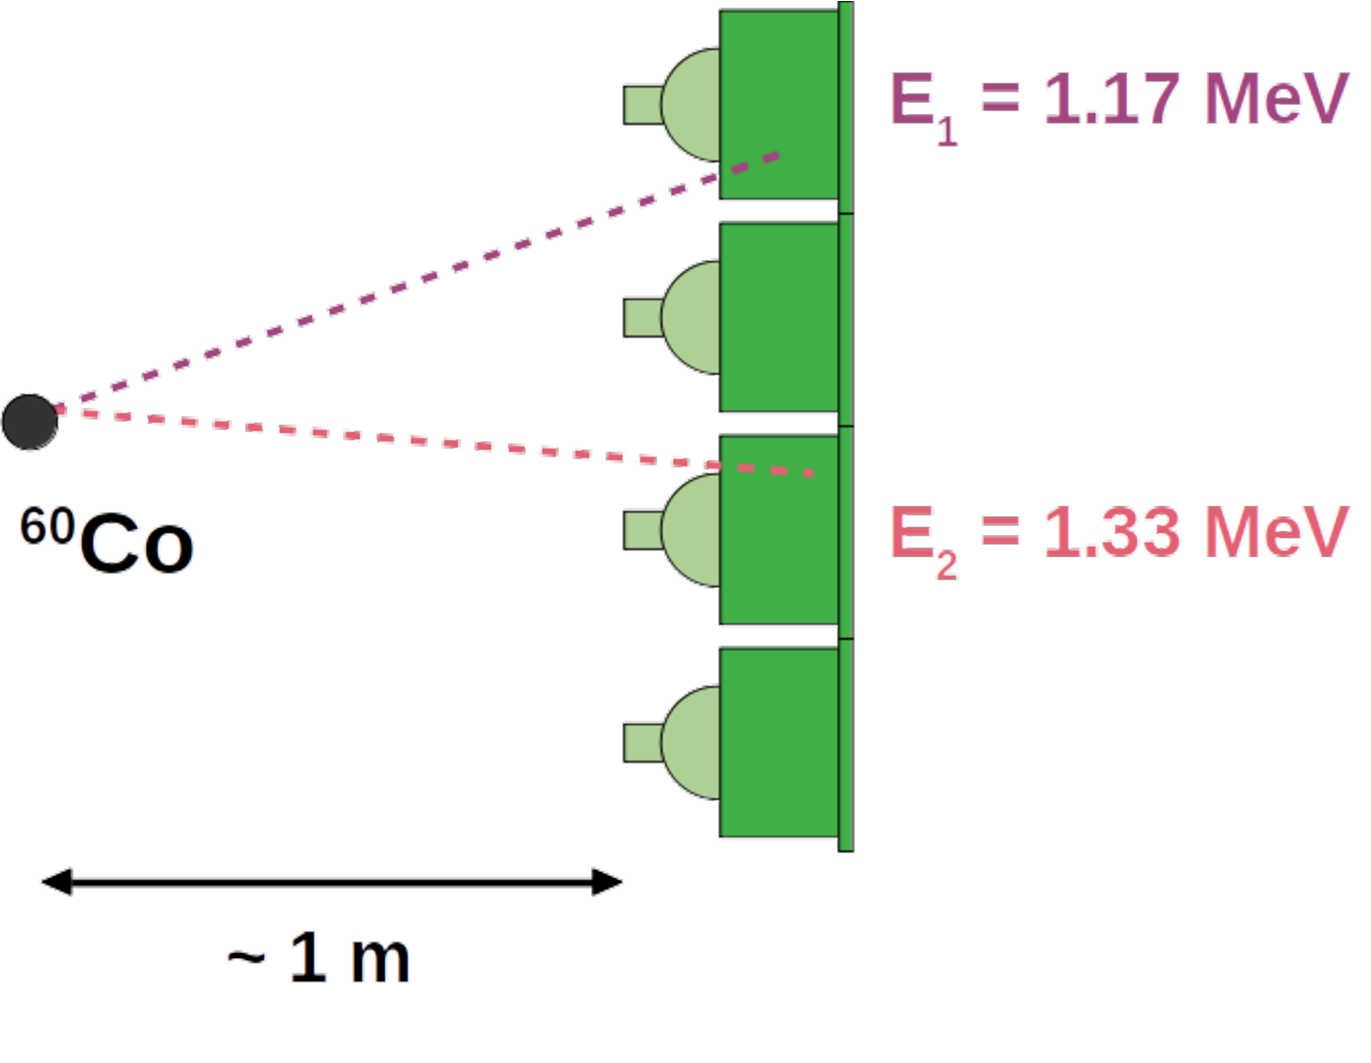
\includegraphics[height=0.5\textwidth]{commissioning/fig_commissioning/Co_setup.pdf}
    \captionsetup{justification=justified}
    \caption{
      \label{subfig:Co_setup}}
  \end{subfigure}
  \hfill
  \begin{subfigure}[t]{0.48\textwidth}
    \centering
    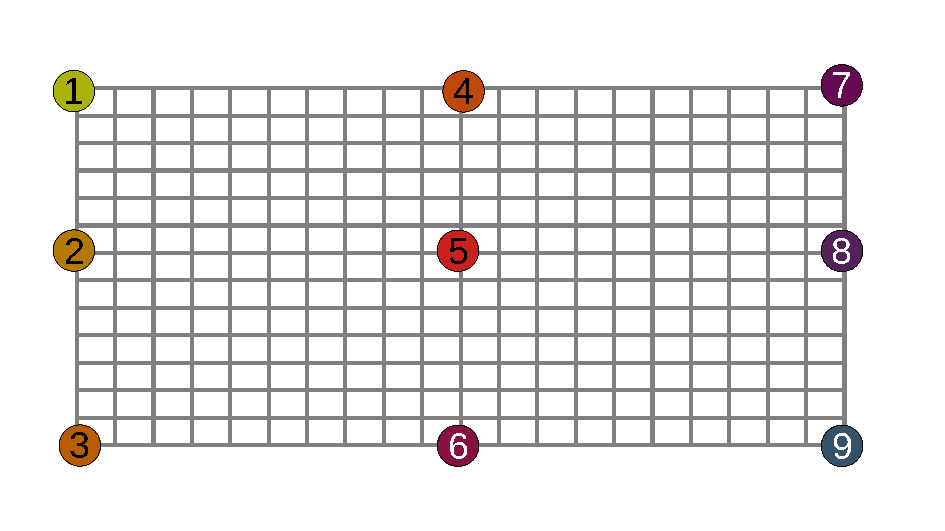
\includegraphics[height=0.5\textwidth]{commissioning/fig_commissioning/Co_setup_wall.pdf}
    \captionsetup{justification=justified}
    \caption{
      \label{subfig:Co_setup_wall}}
  \end{subfigure}
  \caption{(a) Side view example of the Cobalt source positioning behind a calorimeter main wall, schemed by $4$ optical modules (green).
    The emissions of the $2$ $\gamma$'s of interest are displayed in coloured dotted lines.
    (b) Back view of the nine source positions behind a main wall.
    Each grey box represents an optical module.
    \label{fig:Co_exp_design}
  }
\end{figure}
In order for all PMs to detect $\gamma$'s from Cobalt decays, several bunches of data acquisitions were taken:
the source was placed at $9$ different positions on each of the $2$ main calorimeter walls, approximately one meter behind.
Therefore, in total, $19$ data acquisitions have been taken, of which:
\begin{itemize}
\item $18$ with the Cobalt source set behind the wall. The $9$ different positions for one wall are represented in Fig.~\ref{subfig:Co_setup_wall}.
\item $1$ acquisition have been taken without the Cobalt source, with the Italian main wall, to characterise the background detected with the current calorimeter settings.
\end{itemize}
Each data acquisition lasted about $25$ minutes, for a total of $10$ hours of on-site activities, taking into account the time needed to move the Cobalt source from spot to spot.

Currently, the demonstrator is not protected from the laboratory lights by the anti-radon tent.
As laboratory lights would damage the SuperNEMO photomultipliers under tension, two removable black curtains are deployed on top of the detector (that do not interfere with data collection), and acquisitions are taken in dark laboratory.
With this way of doing, all data acquisitions can be performed, while eventual necessary repairs remain possible during the detector commissioning.

Taking acquisitions in the dark is a big constraint.
Moreover, the Cobalt source, initially used for teaching purposes, was loan by IPN laboratory (Orsay), for only two weeks, mainly because of legal constraints.
Therefore, to not disturb LSM on-site activities by plunging the whole laboratory into darkness, and to make the loan time profitable, a SuperNEMO team and I performed night shifts to take data.
The acquisition took place during two weeks, at the summer break $2019$.

\subsubsection*{Simulations and analysis pipelines}

The same way as for the Thallium study discussed in Chapter~\ref{ch:timediff}, all simulations were performed with an ideal calorimeter, setting up the uncertainty on optical modules to zero.
The same Root code was also used to adjust this parameter to the desired value.

As for the data acquisition, the simulated source has been placed behind the calorimeter walls.
Hopefully, there was no need to simulate all the $18$ positions.
In fact, at this time, the detector implemented in simulations is symmetrical in terms of detection performances.
Therefore, simulations of \Co\ events behind the two main walls are equivalent, and we only need to simulate events from $4$ locations (positions $1$, $2$, $4$ and $5$, according to the Fig.~\ref{subfig:Co_setup_wall} numbering system), other being obtained by symmetry operations.
Four bunches, for a total of $10^{9}$ Cobalt events, were simulated with the official Falaise pipeline and stored at the IN$2$P$3$ computing centre platform, making them available to the collaboration.
%% A visualisation, provided by the Falaise Software, of a simulated Cobalt event behind the Italian calorimeter main wall, is shown in Fig.~\ref{fig:Co_visu}.
%% \begin{figure}[h]
%%   \centering
%%   
\includegraphics[width=6cm]{commissioning/fig_commissioning/Co_visu.pdf}
%%   \caption{Visualisation of a simulated Cobalt event.
%%     \label{fig:Co_visu}}
%% \end{figure}

%% \paragraph{Background events simulations:}
%% As already discussed in Chapter~\ref{ch:sensitivity}, currently the collaboration does not supply a complete set of external background simulations for the demonstrator design.
%% This will be implemented as soon as the final demonstrator performances has been determined.
%% Thus, we did not have at our disposal background events simulations for this analysis.

The entire experimental set-up was designed and carried out by me and a group of physicists from LAL, Orsay and LPC, Caen.
I developed a complete set of ROOT codes for data processing and analysis, available on the GitHub platform~\cite{myGit}.
As the tracker is not yet operational for data collection at Modane, we are only interested in the part of the simulations with the calorimeter.
The PID module was therefore not used in the reconstruction pipeline, and other criteria, described in the following sub-section, were used to select the Cobalt events of interest.
A single off-line analysis pipeline has been developed to handle the different output data models of the simulations and real data, in order to ensure the consistency of the analysis.

\subsection{Signal events selection}
\label{subsec:Co_datacut}

We aim to use the two $\gamma$'s of $1.17$ MeV and $1.33$ MeV from Cobalt $60$ $\beta^{-}$ decay, to characterise the time resolutions of individual optical modules.
Thus, the signal we are looking for is two particles detected in coincidence in distinct optical modules.
In order to maximise the signal to background ratio, some selections have been applied on data.
\begin{itemize}
\item Trigger criteria:\\ in the two calorimeter hits channel, the trigger condition is defined so as one of the two hit has to trigger the low energy (or amplitude) threshold, of $50$~keV for the data acquisition.
  As we look for two calorimeter hits, we set an additional off-line selection events whose two hits passed both the high amplitude threshold, corresponding to approximately $150$ keV.
\item Coincidence time criterion:\\ we define the coincidence time-window by events occurring in a $62.5$ ns-long time interval.
  This allows to avoid accidental coincidence events (interactions of two gammas, produced by different sources, in two optical modules), while keeping events where two $\gamma$ particles interact at both ends of the wall.
  This time-window was set for the data-taking and can be improved for eventual future acquisitions.
\item Individual energy selection:\\ in Fig.~\ref{fig:Co_energy_cut} is displayed the hit of highest energy as a function of the one of lowest energy, for simulations with the \Co\ source in position $5$.
  \begin{figure}[h]
    \centering
    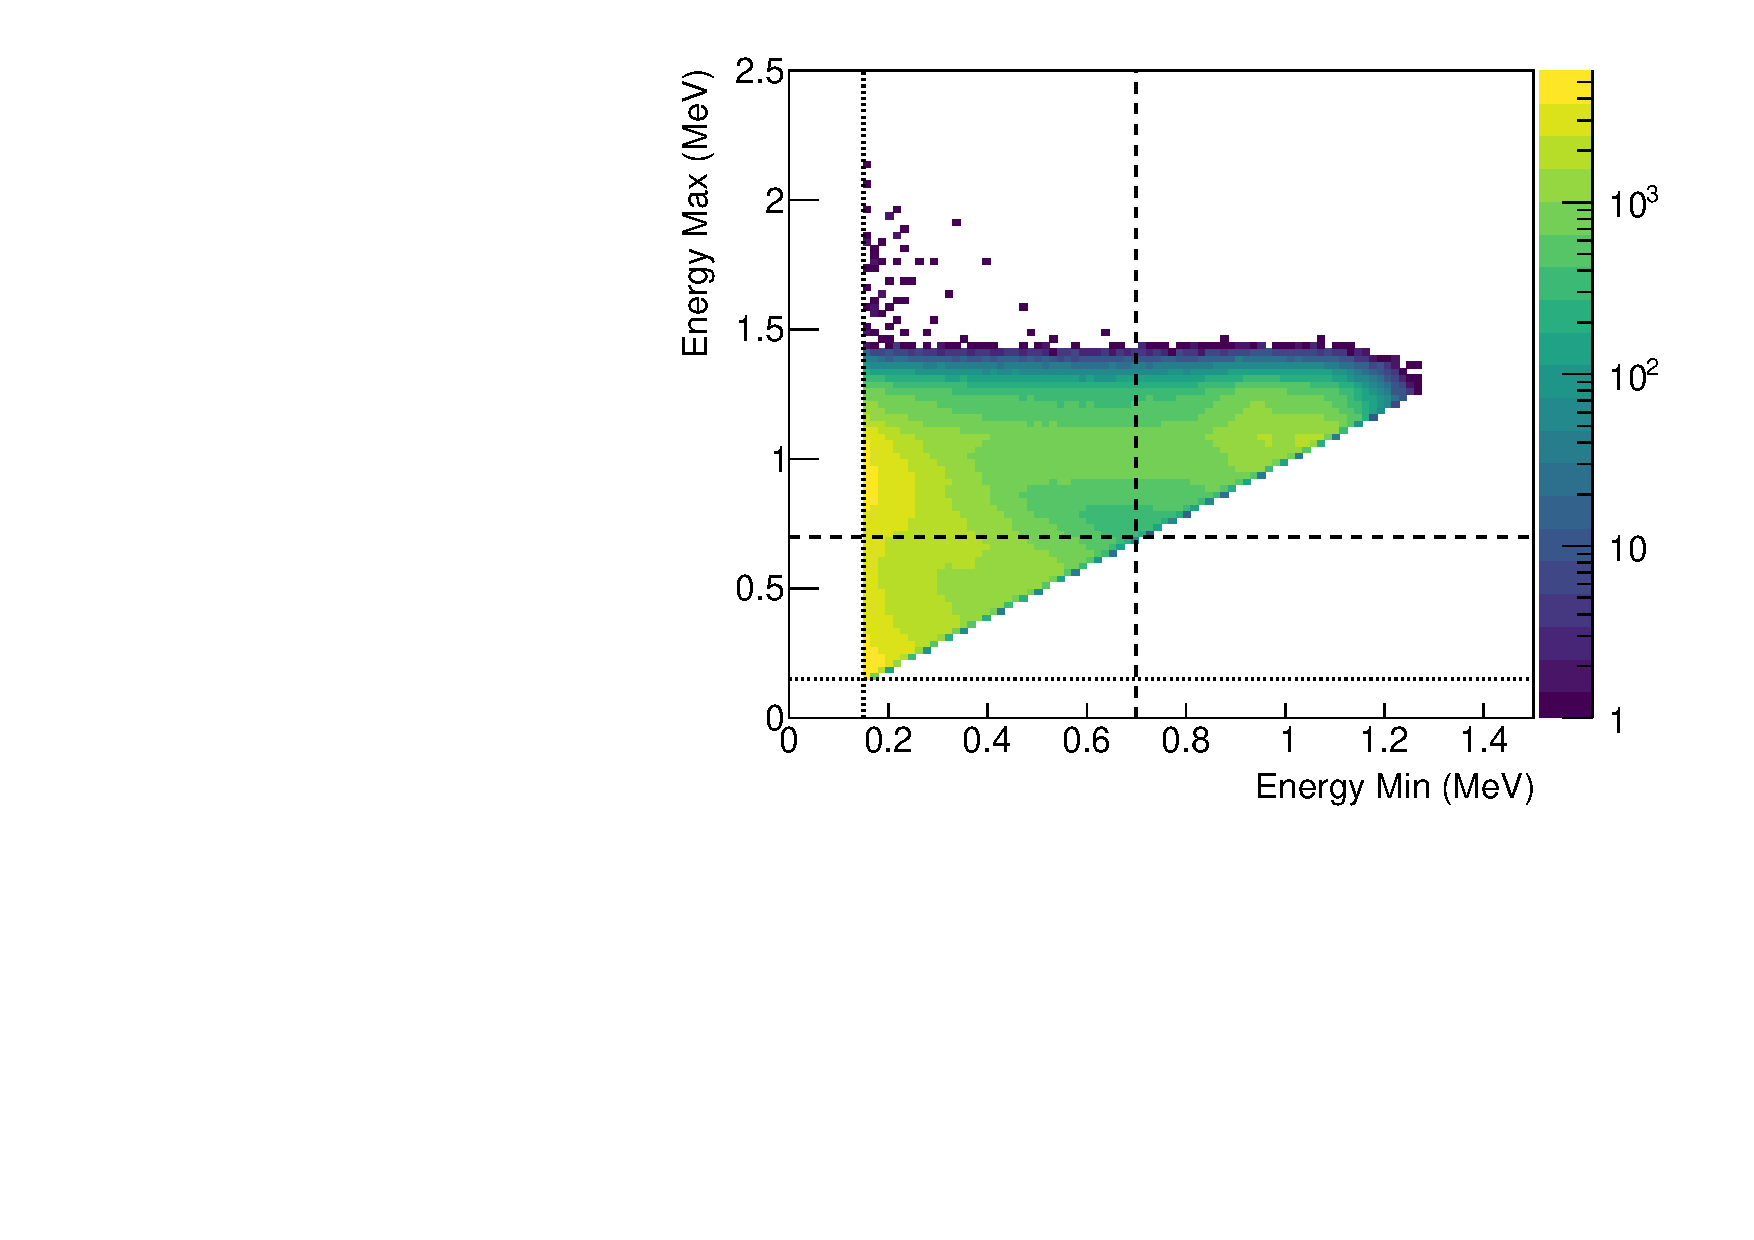
\includegraphics[width=14cm]{commissioning/fig_commissioning/Co_energy_cut.pdf}
    \caption{Maximal energy with minimal energy, for simulated Cobalt events, with source in position $5$ (see Fig.~\ref{subfig:Co_setup_wall}).
      High threshold is represented in black dotted line.
      Dashed lines materialise the individual energy selection.
      \label{fig:Co_energy_cut}}
  \end{figure}
  The high energy threshold is represented by two black dotted lines.
  The topology of interest is observable with two hits around $1$~MeV.
  Also, events where two successive Compton interactions of a single photon from Cobalt occur in two different optical modules are characterised by a high energy hit ($\sim 0.8$ MeV), and a low energy hit ($\sim 0.2$ MeV).
  This topology constitutes a background for this analysis.
  In order to reject them, given the energies of the two interesting Cobalt photons, we only select individual calorimeter hit energies greater than $0.7$ MeV.
  This individual energy selection is pictured by two black dashed lines.
  It naturally highly depends on the calorimeter energy calibration.
  %% If this energy selection is aims to reject \Co\ $\gamma$ particles, but not for background such as \Tl.
\item Geometrical selection:
  with a detector well calibrated in energy, the previous selection is sufficient to prevent double Compton interactions to be selected.
  But, at the time of the data-taking, the detector was not fully calibrated.
  The energy of some reconstructed particle hits then might be badly estimated and some background events could pass this energy selection.
  As such intercations occur predominantly in two close scintillators, we reject topologies where two neighbouring optical modules detect signal in the coincidence window.
  The detector energy calibration is discussed in Sec.~\ref{subsec:Co_energy_calib}.
\end{itemize}
These four selections are intended to improve the Cobalt signal to background ratio.
The coincidence time selection is only applied to real data, while others are applied both to simulations and real data.
Indeed, what we call an \emph{event} does not have the same meaning depending on whether we are talking about simulation or real data.
We simulate a given amount of disintegrations at given location(s) of the detector, so the definition of a Monte Carlo event is straightforward, and concepts such as the pile up has no sense.
For real data acquisitions, a set of criteria have to be established in order to define what an event is, as the time coincidence window for example.

We remind the signification of selection efficiency $\epsilon$ which is
\begin{equation}
  \epsilon = \frac{\text{Number of selected events}}{\text{Total number of events}}\,.
\end{equation}
Selection efficiencies are presented in table~\ref{tab:Co_cut_eff}.
\begin{table}[h]
  \centering
  \begin{tabular}{|c|c|c|c|}
    \hline
    & Simulations & Data \\
    \hline\hline
    High thresold & $35.7$\% & $98.0$\% \\
    Individual energy & $17.0$\% & $70.2$\% \\
    Geometrical & $16.5$\% & $61.0$\% \\
    \hline
  \end{tabular}
  \caption{Selection efficiencies for simulations and real data.
    \label{tab:Co_cut_eff}}
\end{table}
Significant differences are observed between simulations are real data, mainly due to the energy calibration.
Indeed, at the time of the data taking, the gain equalisation and energy calibration were preliminary and had to be improved.
Therefore, this statement directly affect the reconstructed energies of calorimeter hits.
We address this question in Sec.~\ref{subsec:Co_energy_calib}.

%% simus
%% before = 1000001 side = 917239 main = 907700 mult = 35061 event_deltat = 35061


\subsection{Energy calibration}
\label{subsec:Co_energy_calib}

The charge collected at each PM divider is correlated to an energy initially deposited inside the scintillator.
It is important to provide a robust calibration, allowing to provide a relation between these two observables, for any analysis to be valid.
At the time of the data acquisition with the Cobalt source, a complete energy calibration was only provided for data acquisitions taken after the current Cobalt one.
Indeed, as the calorimeter was at the beginning of the commissioning phase, several tests were performed, in particular manipulations that required changing the values of the high voltages.
The equalisation of gains was therefore not yet implemented, which had an impact on the resolution in terms of energy.
In this context, I developped a temporary energy calibration using the data taken with the Cobalt source.

In Fig.~\ref{subfig:Co_calib_charge} is displayed charge spectra for two optical modules located in front of the Cobalt calibration source.
\begin{figure}[h]
  \centering
  \begin{subfigure}[t]{0.8\textwidth}
    \centering
    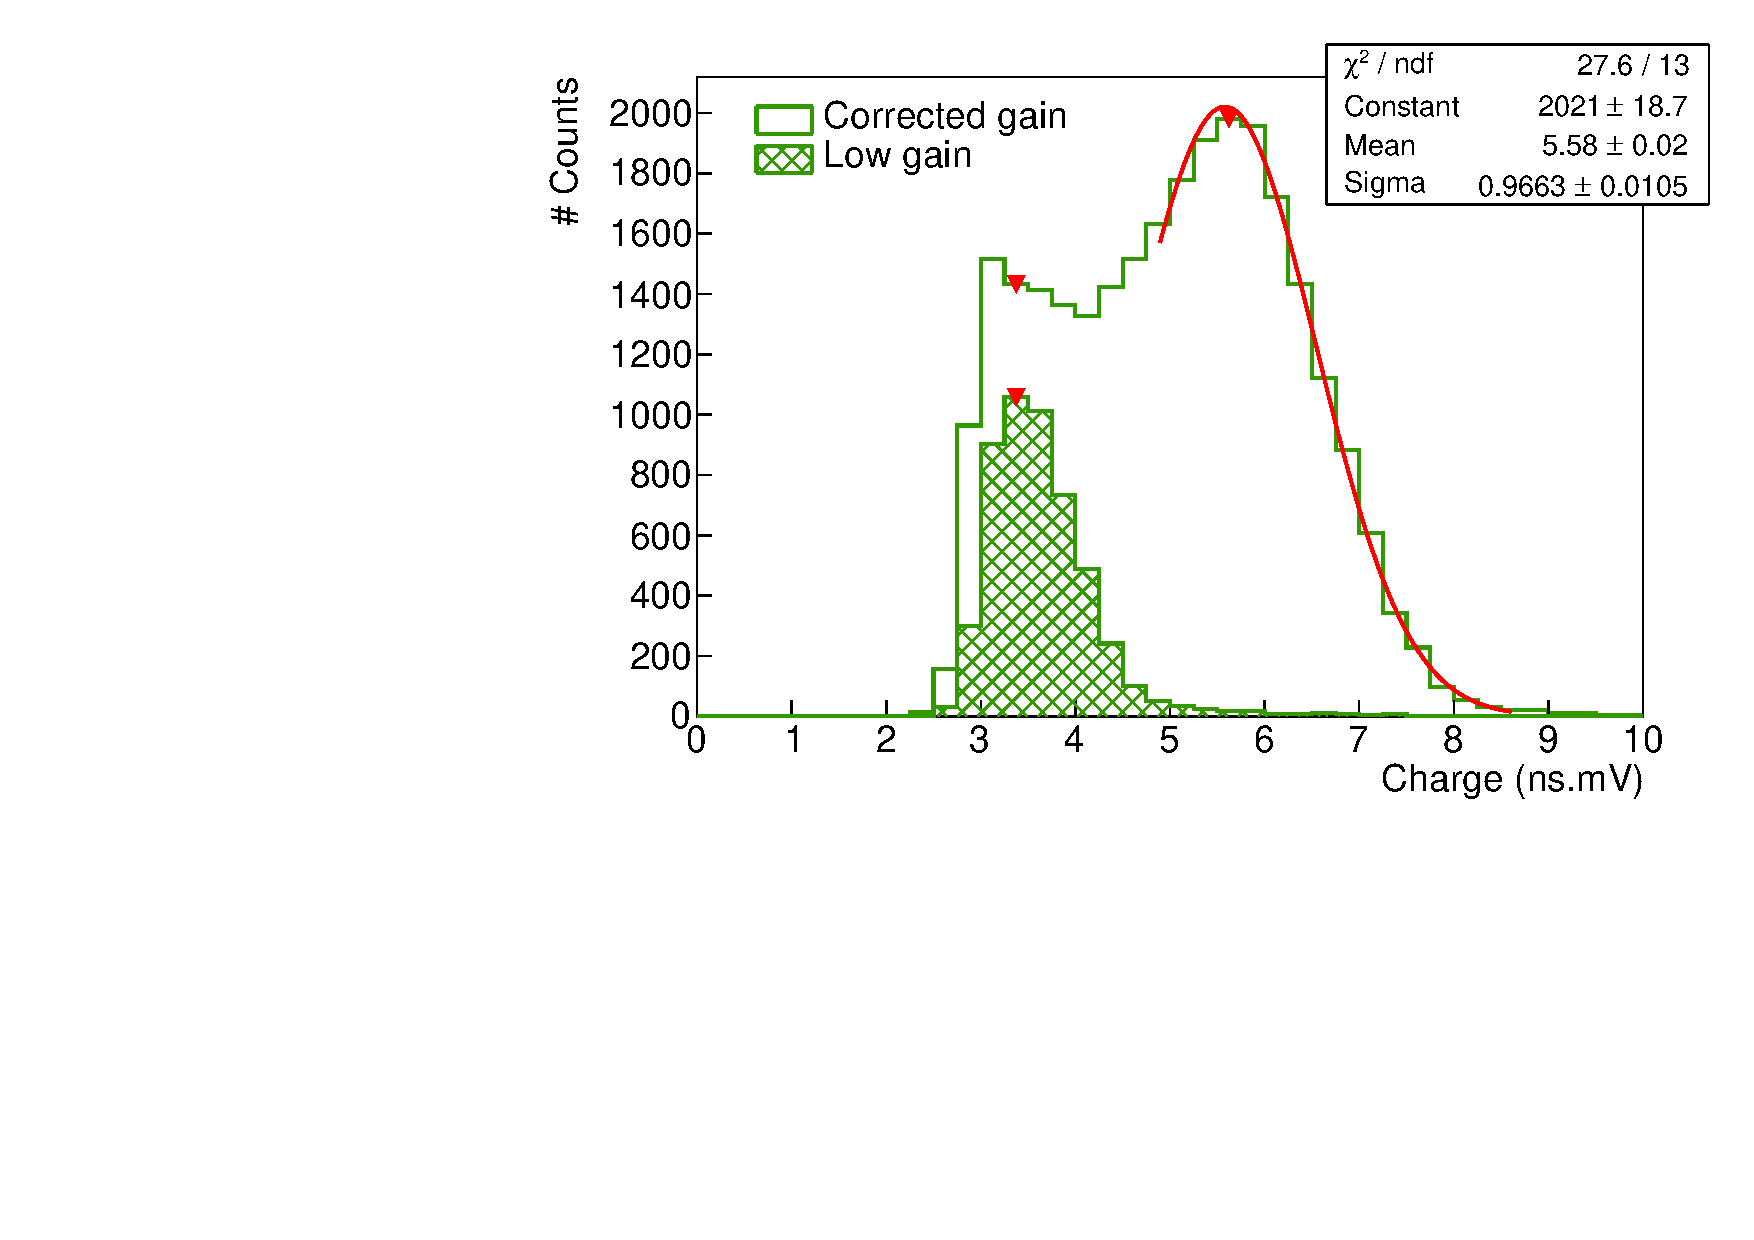
\includegraphics[width=1\textwidth]{CobaltStudy/fig_CobaltStudy/ex_charge_distrib.pdf}
    \captionsetup{justification=justified}
    \caption{Data acquisition.
      \label{subfig:Co_calib_charge}}
  \end{subfigure}
  \hfill
  \begin{subfigure}[t]{0.8\textwidth}
  \centering
  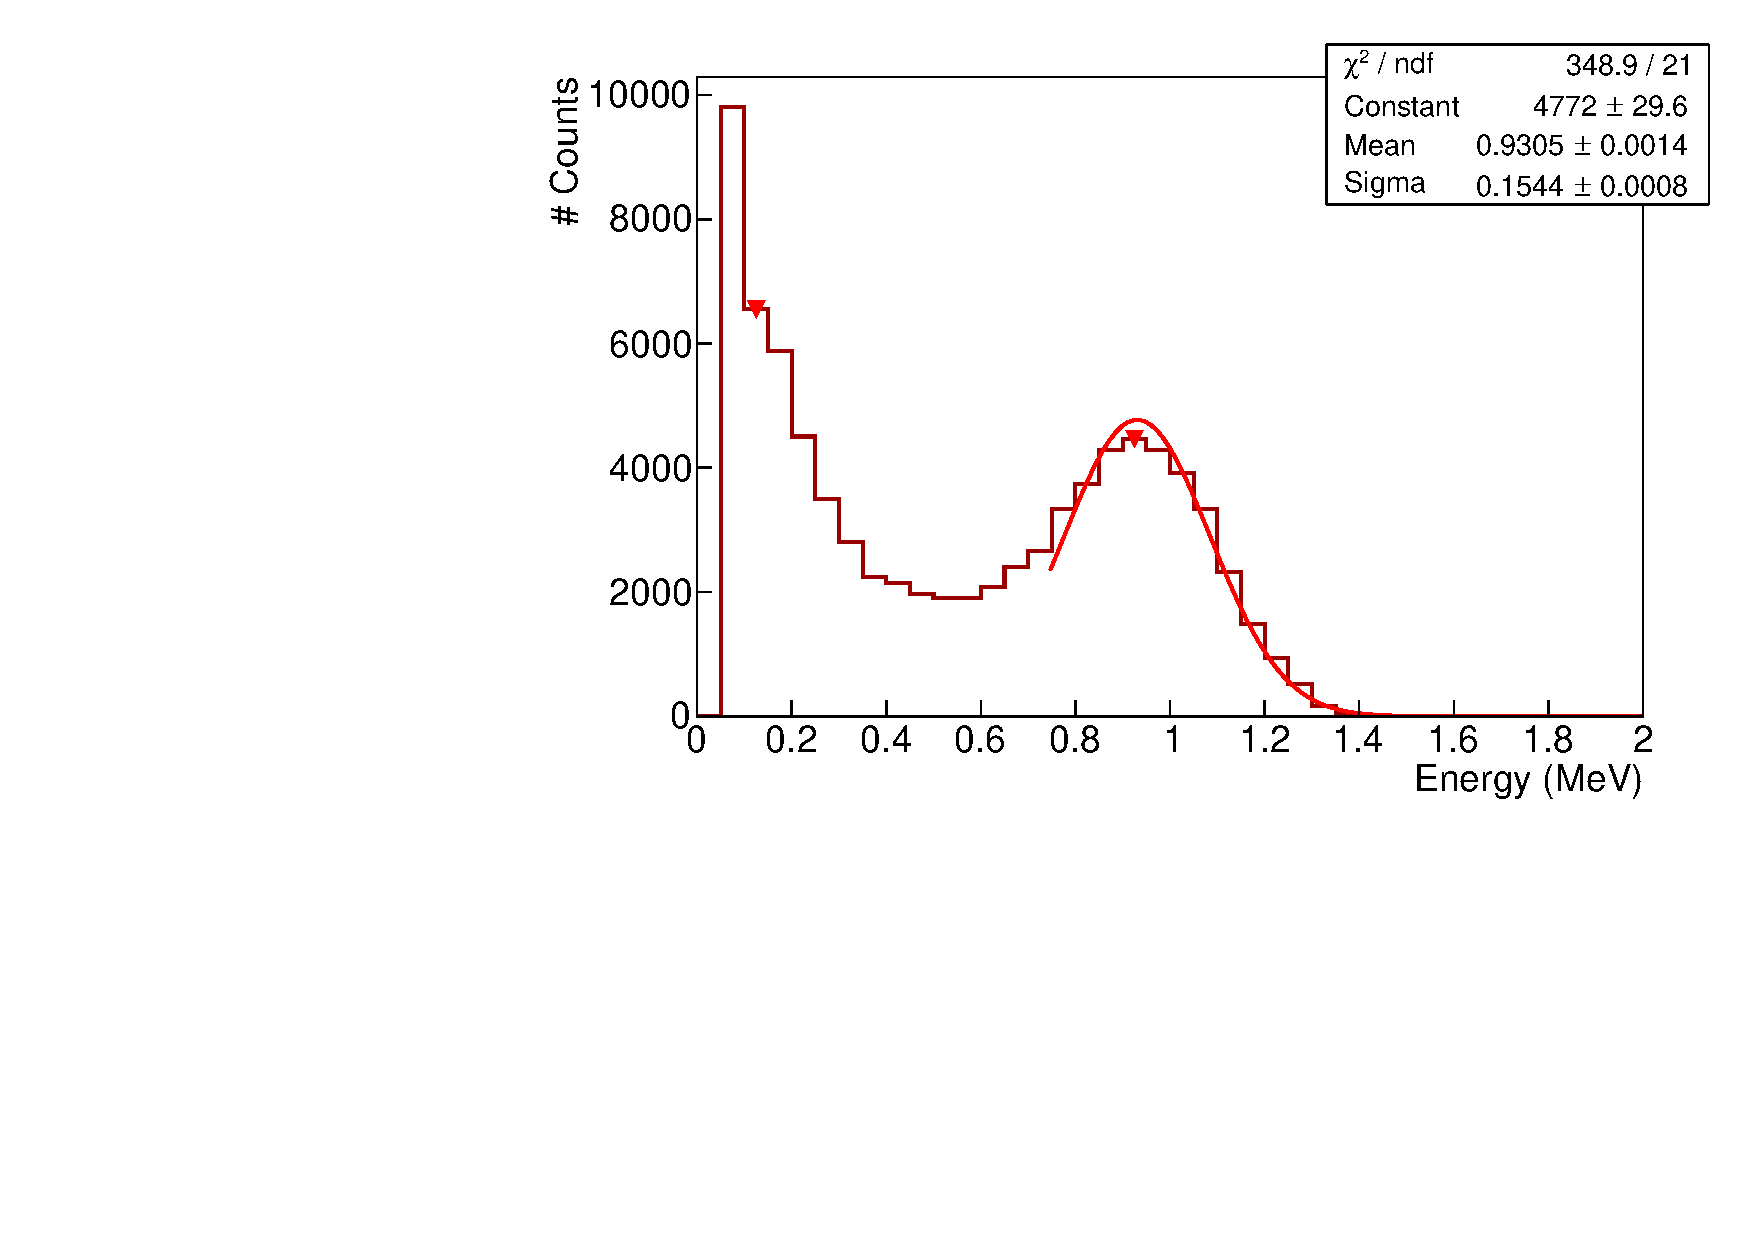
\includegraphics[width=1\textwidth]{CobaltStudy/fig_CobaltStudy/ex_energy_distrib.pdf}
    \captionsetup{justification=justified}
  \caption{Simulated data.
    \label{subfig:Co_calib_energy}}
  \end{subfigure}
  \caption{Data acuqisition charge (a) and simulated energy (b) spectra.
    If two peaks are detected, the second one is fitted with a Gaussian.
    When the OM gain is two low, the first peak is less likely to be detected an the OM is not calibrated.
    \label{fig:Co_calib}}
\end{figure}
In order to have a sufficient statistic, only trigger selection have been applied on data, allowing to select events for which exactly two optical modules triggered (at least one must have triggered the high amplitude threshold).
The first peak is mainly populated by double Compton interactions inside the scintillator, and the second by simple Compton interaction of the two Cobalt $\gamma$'s of interest.
For this energy calibration, the second peak is used as the particular point of the distribution.
An automatic research of the two peaks is performed and, if exactly two peaks are detected, the second one it fitted with a Gaussian function.
This point has been chosen because it is less statistics-dependent than the end point of the distribution.
In the figure, an example of an optical module with an appropriate gain is given, and the fit is well-performed.
An example of an optical module with a too low gain (because it was under a too low high voltage) is also displayed, and shows only one peak.
These kind of distributions were thus no fitted and no energy calibration was provided for them.

The same work is performed on simulated energy distributions for all optical modules.
The fits provide an average of the energy location point corresponding to the second peak, of $0.927\pm0.009$~MeV.
Application of this calibration factor allowed to calibrate $78$ optical modules in total on the French wall.
An energy spectrum of a successfully calibrated optical module is given in Fig.~\ref{fig:calib_energy_OM} after event selection has been applied.
\begin{figure}[h]
  \centering
  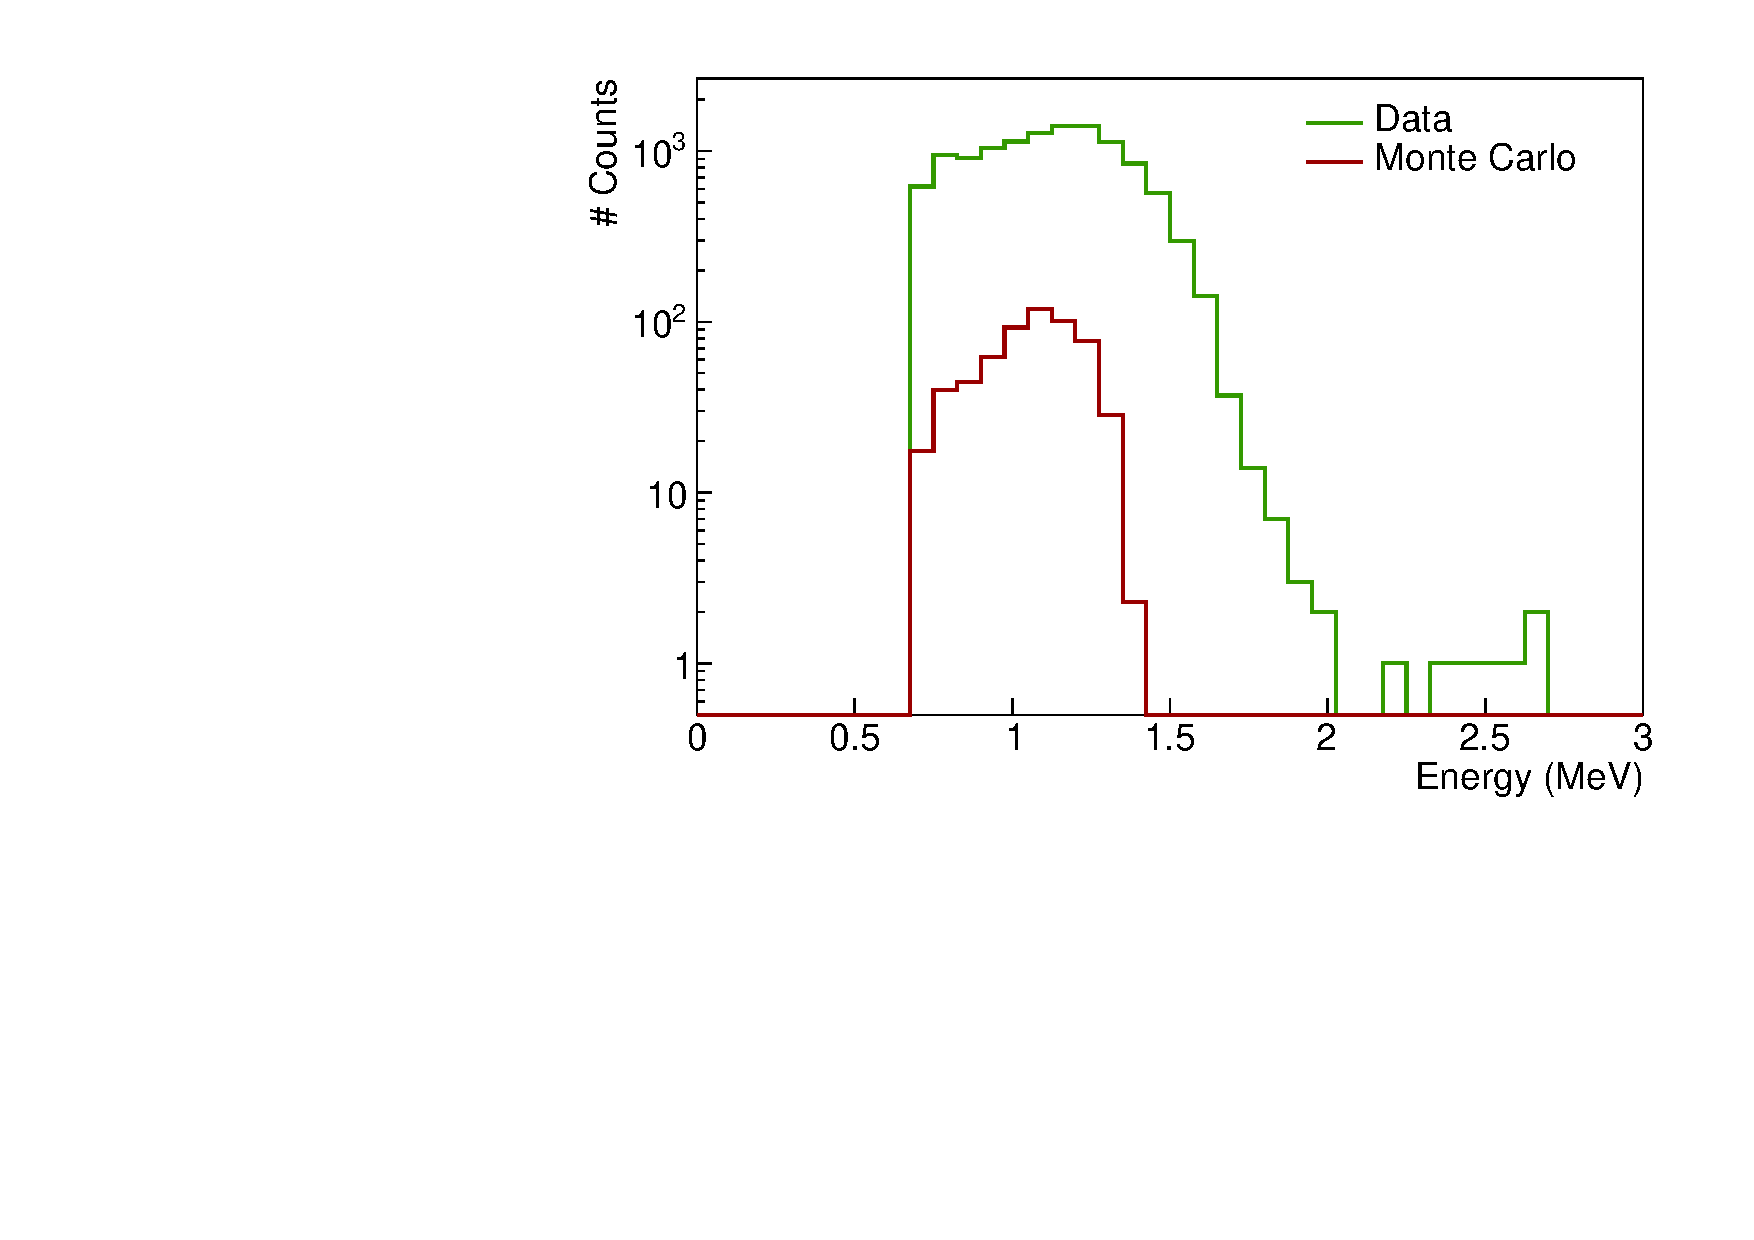
\includegraphics[width=0.8\textwidth]{CobaltStudy/fig_CobaltStudy/calib_energy_done.pdf}
  \caption{Energy spectrum for a calibrated optical module of the French wall, using Cobalt data acquisition.
    The simulations have been normalised to the source activity and data acquisition time.
    \label{fig:calib_energy_OM}}
\end{figure}
We find the results obtained in the previous sub-section concerning the difference in efficiency between simulations and real data.
This will be improved by new data acquisitions that will be taken during the month of November, because all optical modukes are now equalised in gain.
We also notice that the data spectrum extends at higher energies than simulations, corresponding to the \Tl\ background as well as external $\gamma$'s.

Selection efficiencies for each cut-off, after the energy calibration, are given in Tab.~\ref{tab:Co_cut_eff_calib}.
\begin{table}[h]
  \centering
  \begin{tabular}{|c|c|c|c|}
    \hline
    & Simulations & Data \\
    \hline\hline
    High thresold & $35.7$\% & $94.0$\% \\
    Individual energy & $17.0$\% & $58.0$\% \\
    Geometrical & $16.5$\% & $51.9$\% \\
    \hline
  \end{tabular}
  \caption{Selection efficiencies for simulations and real data.
    Energy calibration with Cobalt data have been applied.
    \label{tab:Co_cut_eff_calib}}
\end{table}
We notice an improvement at the level of individual energy cut, where the selection efficiency is reduced compared with the previous case using the energy calibration provided by the collaboration.

This is a temporary calibration, only use in the framework of this analysis, and does not replace the more complete one accomplished for later data acquisitions.
An amelioration could be brougth with a double gaussian fit on the two peaks.
Nervertheless, this improvement is not necessary since the gains were not yet aligned.
But it will be interesting to try this method again with the new Cobalt data.


\subsection{Background estimation}
\label{subsec:bkg_estimation}

The signal for this analysis is composed two $\gamma$'s of $1.17$ MeV and $1.33$ MeV, emitted after Cobalt disintegrations.
After application of the four selections, it is primordial to estimate and characterise the remaining background in the selected topology, detected by the calorimeter during the data acquisition.

\subsubsection*{Types of background}

Mainly three different types of background can be harmful for this analysis, all pictured in Fig.~\ref{fig:Co_bkg}.
\begin{figure}[h]
  \centering
  \begin{subfigure}[t]{0.30\textwidth}
    \centering
    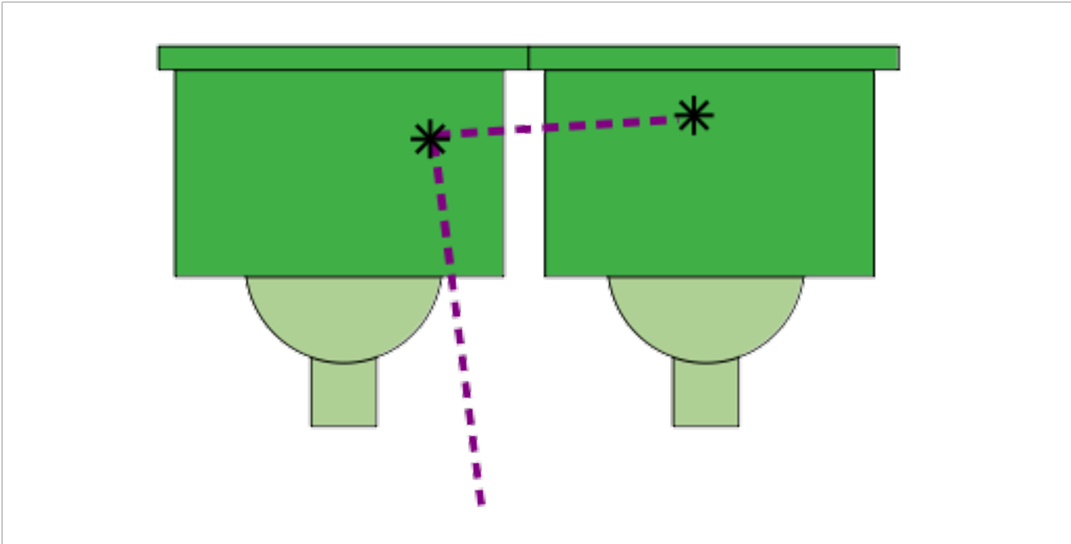
\includegraphics[height=0.50\textwidth]{commissioning/fig_commissioning/Co_bkg_1.pdf}
    \captionsetup{justification=justified}
    \caption{
      \label{subfig:Co_bkg_1}}
  \end{subfigure}
  \hfill
  \begin{subfigure}[t]{0.30\textwidth}
    \centering
    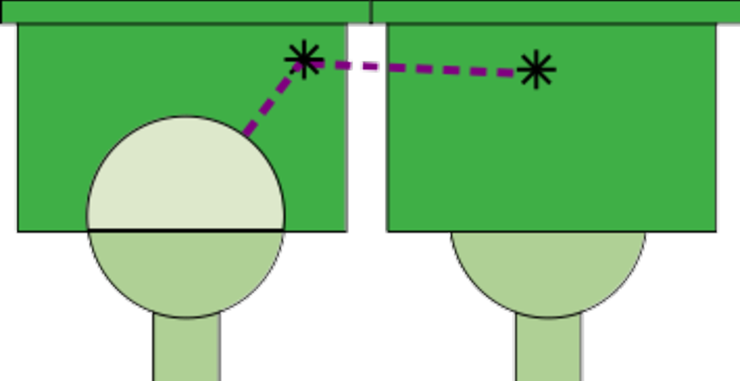
\includegraphics[height=0.50\textwidth]{commissioning/fig_commissioning/Co_bkg_2.pdf}
    \captionsetup{justification=justified}
    \caption{
      \label{subfig:Co_bkg_2}}
  \end{subfigure}
  \hfill
  \begin{subfigure}[t]{0.30\textwidth}
    \centering
    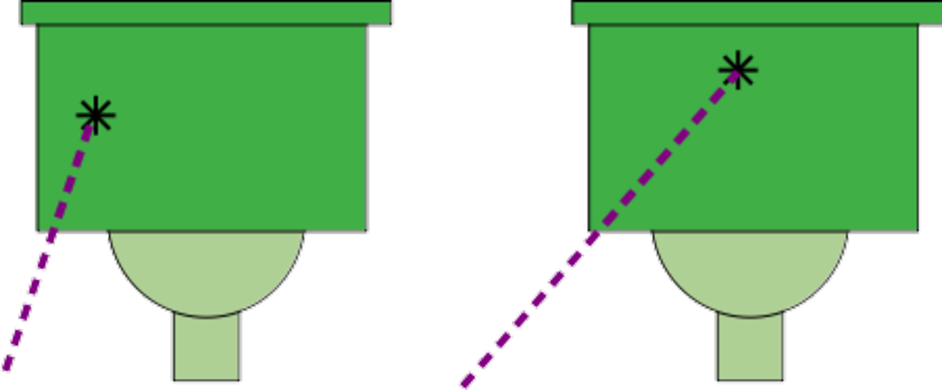
\includegraphics[height=0.50\textwidth]{commissioning/fig_commissioning/Co_bkg_3.pdf}
    \captionsetup{justification=justified}
    \caption{
      \label{subfig:Co_bkg_3}}
  \end{subfigure}
  \caption{Background types for the Cobalt study.
    Interactions of photons in scintillators are represented by black stars.
    (a) Interaction of a single Cobalt photon in two scintillators through double Compton scattering.
    (b) Interaction of a photon coming from natural radioactive isotopes contamination (PM glass...), through double Compton scattering.
    (c) Interactions of two uncorrelated photons, coming from the demonstrator outside (natural radioactivity of laboratory rock...), in two scintillator blocks
    \label{fig:Co_bkg}}
\end{figure}
\begin{itemize}
\item Through a double Compton interaction, a single Cobalt $\gamma$ particle can deposit energy in two scintillator blocks (see Fig.~\ref{subfig:Co_bkg_2}).
As described in Sec.~\ref{subsec:Co_datacut}, the geometrical and individual energy selections have been set up to reject these background events.
\item Photons coming from the natural radioactive decay chains of $^{238}$U, $^{232}$Th and $^{40}$K isotopes.
Typically, the $2.61$ MeV-$\gamma$, from \Tl\ decay, can interact successively in two scintillators through Compton scatterings and produce high energy events (see Fig.~\ref{subfig:Co_bkg_1}).
These disintegration can occur in the source foils or in the detector's components (mainly PM glass).
\item At the time of the data acquisition, the calorimeter was in commissioning phase, and the iron shielding was not yet installed.
Therefore, the calorimeter was not properly protected from external particles, coming from outside the detector (radioactive isotope contamination of laboratory rock).
Accidental events where two decorrelated $\gamma$ particles, can be detected in two scintillator blocks (see Fig.~\ref{subfig:Co_bkg_3}).
The coincidence time window should avoid these accidental to be selected.
\end{itemize}
All these three topologies can mimic the Cobalt two-$\gamma$'s signal.

Estimating the amount of background received by optical blocks during the acquisition is essential to assess our results.
In order to characterise the two last types of background (decorrelated from the Cobalt source), an acquisition without the Cobalt calibration source has been performed (see Sec.\ref{subsec:Co_setup}).
Unfortunately, be owing to optical modules gain issues, these data are not usable.
Therefore, we use the data acquisition taken with the Cobalt source set behind the wall to estimate this background.

\subsubsection*{Background characterisation}

When the Cobalt source is set behind the wall, collected data may contain signal events coming from it as well as background events.
Let us assume these background events are dominated by radiocative decays and external $\gamma$'s, by considering the background coming from double Compton intercations of Cobalt $\gamma$'s have been efficiently removed by application of the individual energy cut.
We choose to modelise the Cobalt data as a linear combination of signal events $s$ and background events $b$
\begin{equation}
  \hat{d}=s+b\,,
  \label{eq:estimation_data}
\end{equation}
where $s$ and $b$ are thus considered as uncorrelated.
The question is how to extract informations about background, using the Cobalt data acquisitions?
We remind the Cobalt source was placed at different positions behind the calorimeter wall (Fig.~\ref{subfig:Co_setup_wall}, Sec.~\ref{subsec:Co_setup}).
We aim to take advantage of those different configurations to reach our goal.
In the following, we make use of the positions $2$ and $8$ for the Cobalt source.
Therefore, depending on whether the source is in one of the two positions, some optical modules are \emph{close} to it, others are \emph{far}.
More precisely, we consider as \emph{close}, the optical modules that are separated from the source by less than 10 OMs (i.e. less than half the wall-lenght), the others being \emph{far} from it\footnote{For example, an optical module located on the left (right) of the calorimeter wall, is considered as far from (close to) the source, if the source is in position $8$.}.
Considering that, we distinguish two categories of data, $\hat{d}^{\,\text{close}}$ and $\hat{d}^{\,\text{far}}$, defined as the estimations of data events detected by an optical module when the source is close to, or far from it, respectively.
Then, we precise our data modelisation with
\begin{equation}
  \hat{d}^{\,\text{close}} = b + s^{\,\text{close}}\,,
  \label{eq:estimation_data_close}
\end{equation}
where $s^{\,\text{close}}$ is naturally the number of signal Cobalt events detected by a given optical module for which the distance from the source, $D_{\,\text{source}}$, is lower than $10$.
In the same way, considering $s^{\,\text{far}}$ as signal events detected by an optical module from which the source is far, we have
\begin{equation}
  \hat{d}^{\,\text{far}} = b + s^{\,\text{far}}\,.
  \label{eq:estimation_data_far}
\end{equation}
Estimations of $s^{\,\text{close}}$ and $s^{\,\text{far}}$ (respectively noted $\tilde{s}^{\,\text{close}}$ and $\tilde{s}^{\,\text{far}}$) are provided using simulations of \Co\ events in positions $2$ or $8$.
Indeed, as we consider the double Compton interaction background as negligible, the amount of signal events received for optical modules far or close from the source can be established with Cobalt simulations.
Then, the coefficient $\alpha$ defined as
\begin{equation}
  \alpha = \tilde{s}^{\,\text{far}}/\tilde{s}^{\,\text{close}}\,.
\end{equation}
It depends on the distance $D_{\,\text{source}}$ and is found to be $0.05 \% < \alpha < 5 \%$, meaning that the number of simulated signal events detected by optical modules distant from the source is greatly lower than for close optical modules, for a given source position.

In order to provide a non-biased estimation of $b$ given the data model in Eq.~\eqref{eq:estimation_data_far}, we would remove $\tilde{s}^{\,\text{far}}$, estimated through simulations, from $\hat{d}^{\,\text{far}}$, which can be estimated with Cobalt data acquisition.
%%on voudrait avoir b=dfar, mais c'est biaisé pcq il reste signal. On pourrait enlever sfar, mais
%%c'est la merde de faire ça avec les simus
To do so, we display in Fig.~\ref{fig:Co_data_bkg} the number of calorimeter hits, after event selection, counted by each optical module, as a function of the distance to the Cobalt source.
\begin{figure}[h]
  \centering
  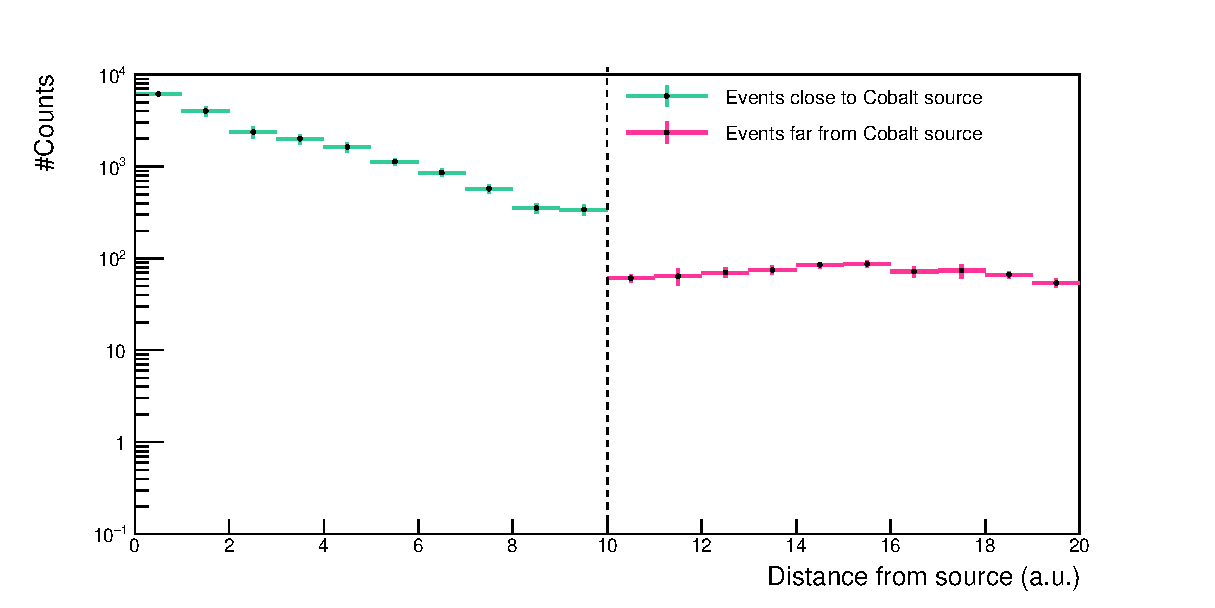
\includegraphics[width=1.1\textwidth]{commissioning/fig_commissioning/Co_data_bkg.eps}
  \caption{Number of events for pairs of OMs close and far from the source, for real data (orange) and simulated data (blue), as a function the distance to the source (in units of number of OM).
    The vertical dashed line materialises the distance limit of $10$ OMs from the source.
    \label{fig:Co_data_bkg}}
\end{figure}
The $10$ OMs limit is materialised by a vertical dashed line.
Calorimeter hits that occurred in coincidence above and below this limit are displayed both for simulated and real data.
Therefore, events where the two hits occur in two optical modules, each located in one half of the calorimeter, are not represented.
This explains the observable gap at the $10$ OMs limit level.

We first focus on simulation results.
Calorimeter hits for which $D_{\,\text{source}}<10$, represent the estimation of the amount of signal events detected close to the source, $\tilde{s}^{\,\text{close}}$.
Similarly, hits for which $D_{\,\text{source}}>10$ embed for $\tilde{s}^{\,\text{far}}$, the amount of signal events remaining for optical modules far from the calibration source site.
As expected, the number of signal Cobalt events decreases with the distance to the source.
Moreover, this decrease is linear, showing the same slope beyond and above the $10$ OMs limit.

Regarding real data acquisition, calorimeter hits for which $D_{\,\text{source}}<10$ materialise the number of data events estimation $\hat{d}^{\,\text{close}}$.
Apart from slight differences due to the detector efficiency, these data events follow the same linear evolution as signal events with the distance to the source.
This leads us to conclude that optical modules close to the source are dominated by Cobalt signal events.
Similarly, $D_{\,\text{source}}>10$ events stand for $\hat{d}^{\,\text{far}}$.
We observe that $\tilde{s}^{\,\text{far}}/\hat{d}^{\,\text{far}} \ll 1$, which is compatible with the $\alpha$ coefficient values, being $5\%$ in the worse case, explaining the few amount of $\tilde{s}^{\,\text{far}}$ events remaining for optical modules far from the source.
Moreover, we find that the amount of $\hat{d}^{\,\text{far}}$ events is globally stable with the distance to the source, which confirms the assumption made that, at such distances from the source, radioactive contaminant decays and external $\gamma$'s interactions dominate the background contribution and are decorrelated from the Cobalt source.
%% donc bkg qui ne vient pas de la source
Therefore, for a $25$ minutes run, each optical module detects around $10^{2}$ external background events.
%% différence data/simus dans close : gain equalization ptetre pas dégueu sinon on verrait une diff
%% à ce niveau là. gain equalisation of optical modules, discussed in Sec.~\ref{sec:comm_energy_calibration}, could impact greatly the .

To sum up these results, calorimeter hits for optical modules close to the Cobalt calibration source are, for the most part, signal events.
Besides, hits occurring far from the source are predominantly background events.
As we moved the source in different positions, we have access to the estimation of background rate $\hat{b}$ for each optical module (when the source is far), and to the estimation of $\hat{s}$ (when the source is close).
Therefore, we can compute the signal to background ratio, as a function of the distance to the Cobalt source, displayed in Fig.~\ref{fig:Co_ratioSB}.
\begin{figure}[h]
  \centering
  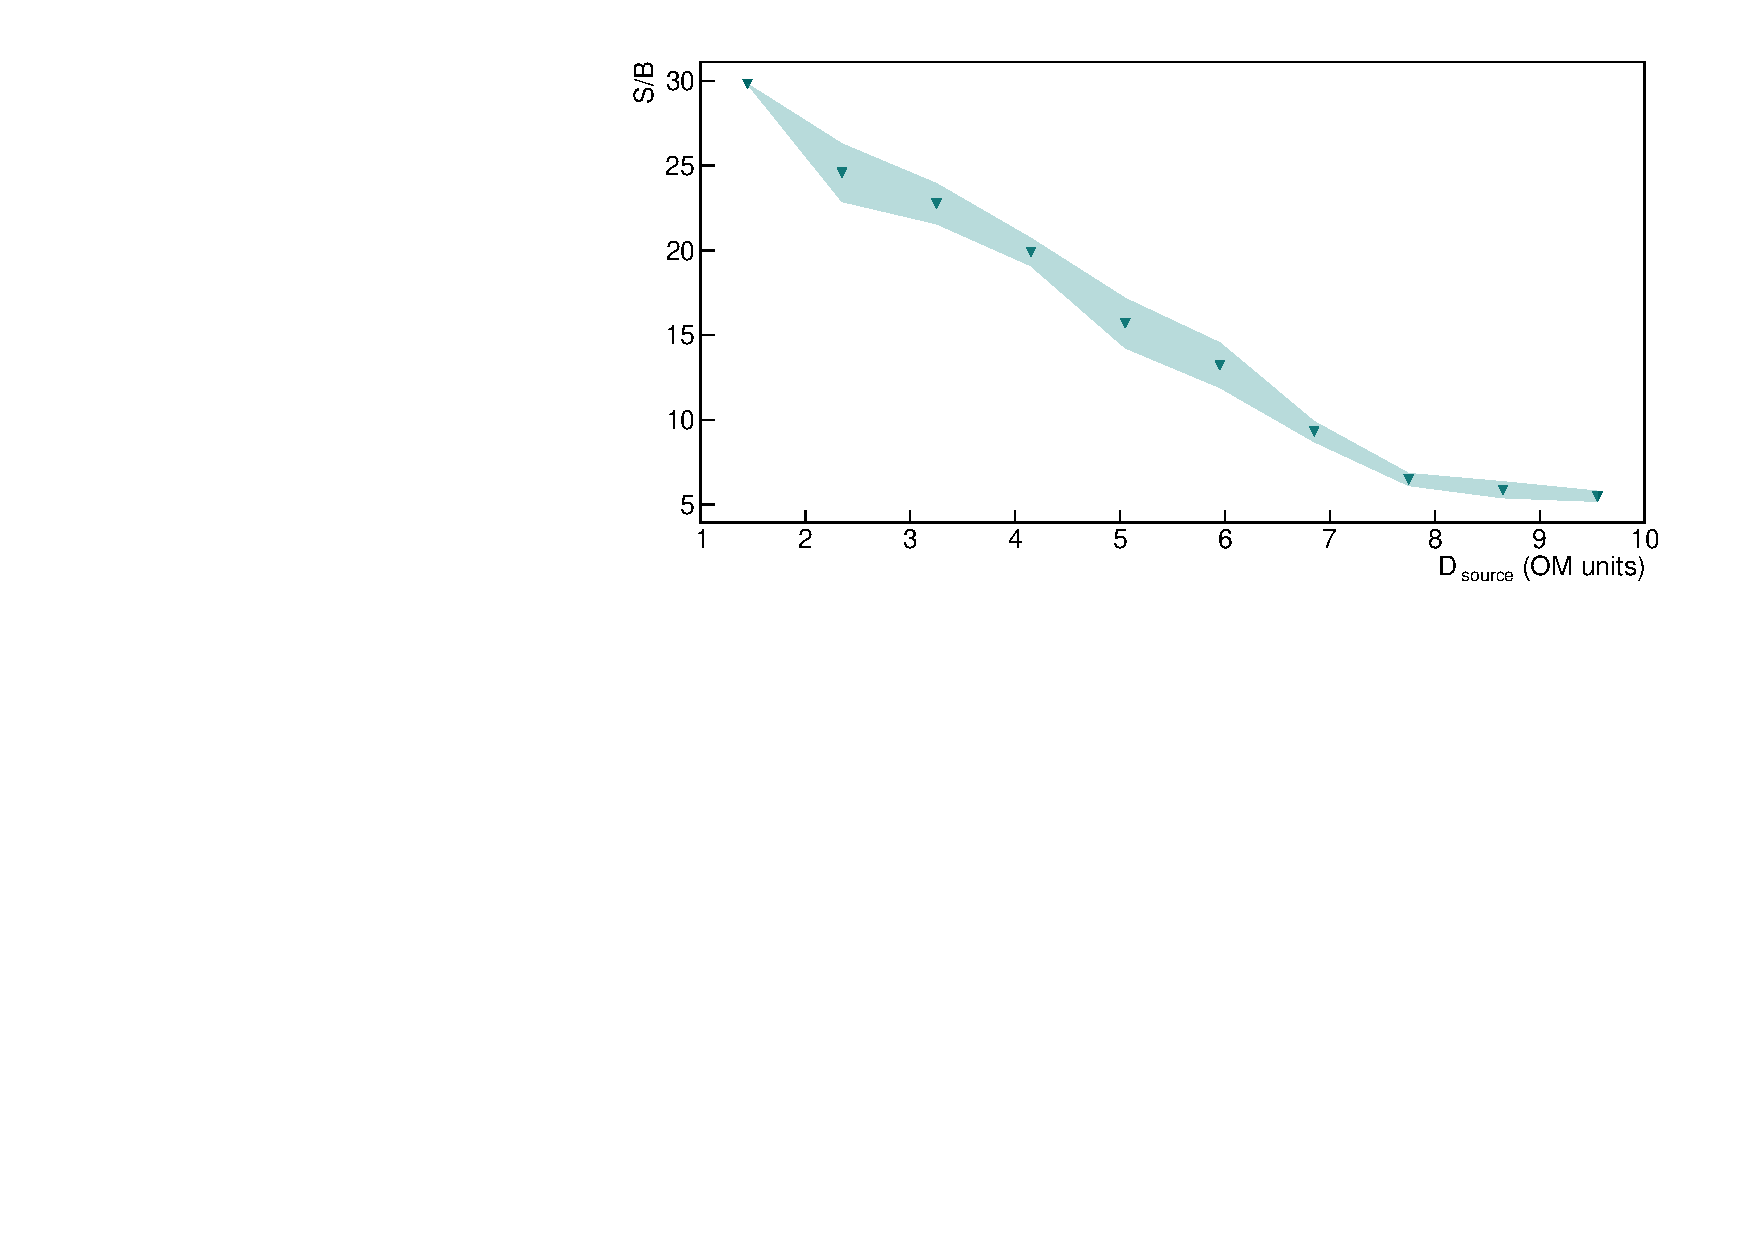
\includegraphics[width=1.1\textwidth]{commissioning/fig_commissioning/Co_ratioSB_distance.pdf}
  \caption{Signal to background ratio for each optical module, as a function of the distance to the Cobalt source.
    \label{fig:Co_ratioSB}}
\end{figure}
The number of signal events in each optical module depends on the distance to the source, which is not the case for the number of background events, explaining the decreasing of $S/B$ with $D_{\,\text{source}}$.
For this reason, the distribution stabilises at high $D_{source}$ ($\sim8$ OM units) as these optical modules are more sensitive to the flat background contribution than those right in front of the source.
%% on mesure alpha et il est petit donc on peut négliger sfar dans la modélisation

To summarise, in this subsection, we gave informations on background events for the whole French wall, using data taken with the Cobalt source set at different positions.
We confirmed our assumption that the more one optical block is far from the source, the less it detects $\gamma$ particles emitted after Cobalt disintegrations, then the more the signal to background ratio decreases.
In the following, in order to properly compare simulated and real data, we give an order of magnitude of the detector efficiency during the data-taking with the Cobalt source.

%% faut dire que du coup on peut croire nos résultats quand la source est proche pour l'analyse time reso
%% aussi : Remarque : dans la suite (mesure des sigma_t), tu pourrais faire l'analyse pour les blocs
%% qui vérifient S/B > 10

%% dire qu'on peut faire ça avec d'autres runs mais que c'était pour avoir un ordre d'idée

%%Remarque : le bruit de fond peut décroitre sur les bords - ex : 2-3 dernières colonnes de PM (et
%%c'est un peu ce que tu vois sur la figure 7.8)

%% *Dire que ç'aurait été mieux de prendre un OM de ref pcq là on moyenne mais pas poss car pas de stat*
%% * finir: l'idée c'est de dire sortir un spectre en énergie data+estimation du bdf avec ce qu'on vient de faire.
%% Je vais prendre toutes les paires d'OMs possibles pour les OMs loin de la source, et tracer leur spectre en énergie en coincidence.
%% ça va me donner un histogramme binné sur l'énergie, et chaque bin aura une certaine dispersion, qui vient des différences des spectres en énergie des OMs\\



%% \subsection{Detector efficiency}
%% \label{subsec:detector_efficiency}

%% %% parler de la baisse d'eff du à la saturation de l'acqu
%% %% *A mettre quelque part:
%% %% the energy calibration discussed in Sec.~\ref{sec:comm_energy_calibration} was not completed, and optical modules' gains were not all aligned.*


%% Standing as an example, we compare real and simulated energy spectra for a given pair of optical modules detecting events in coincidence.
%% We provide these spectra in Fig.~\ref{fig:detector_efficiency}, where events satisfy to the four criteria described in Sec.~\ref{subsec:Co_datacut}, for the Cobalt source in position $5$.
%% \begin{figure}[h]
%%   \centering
%%   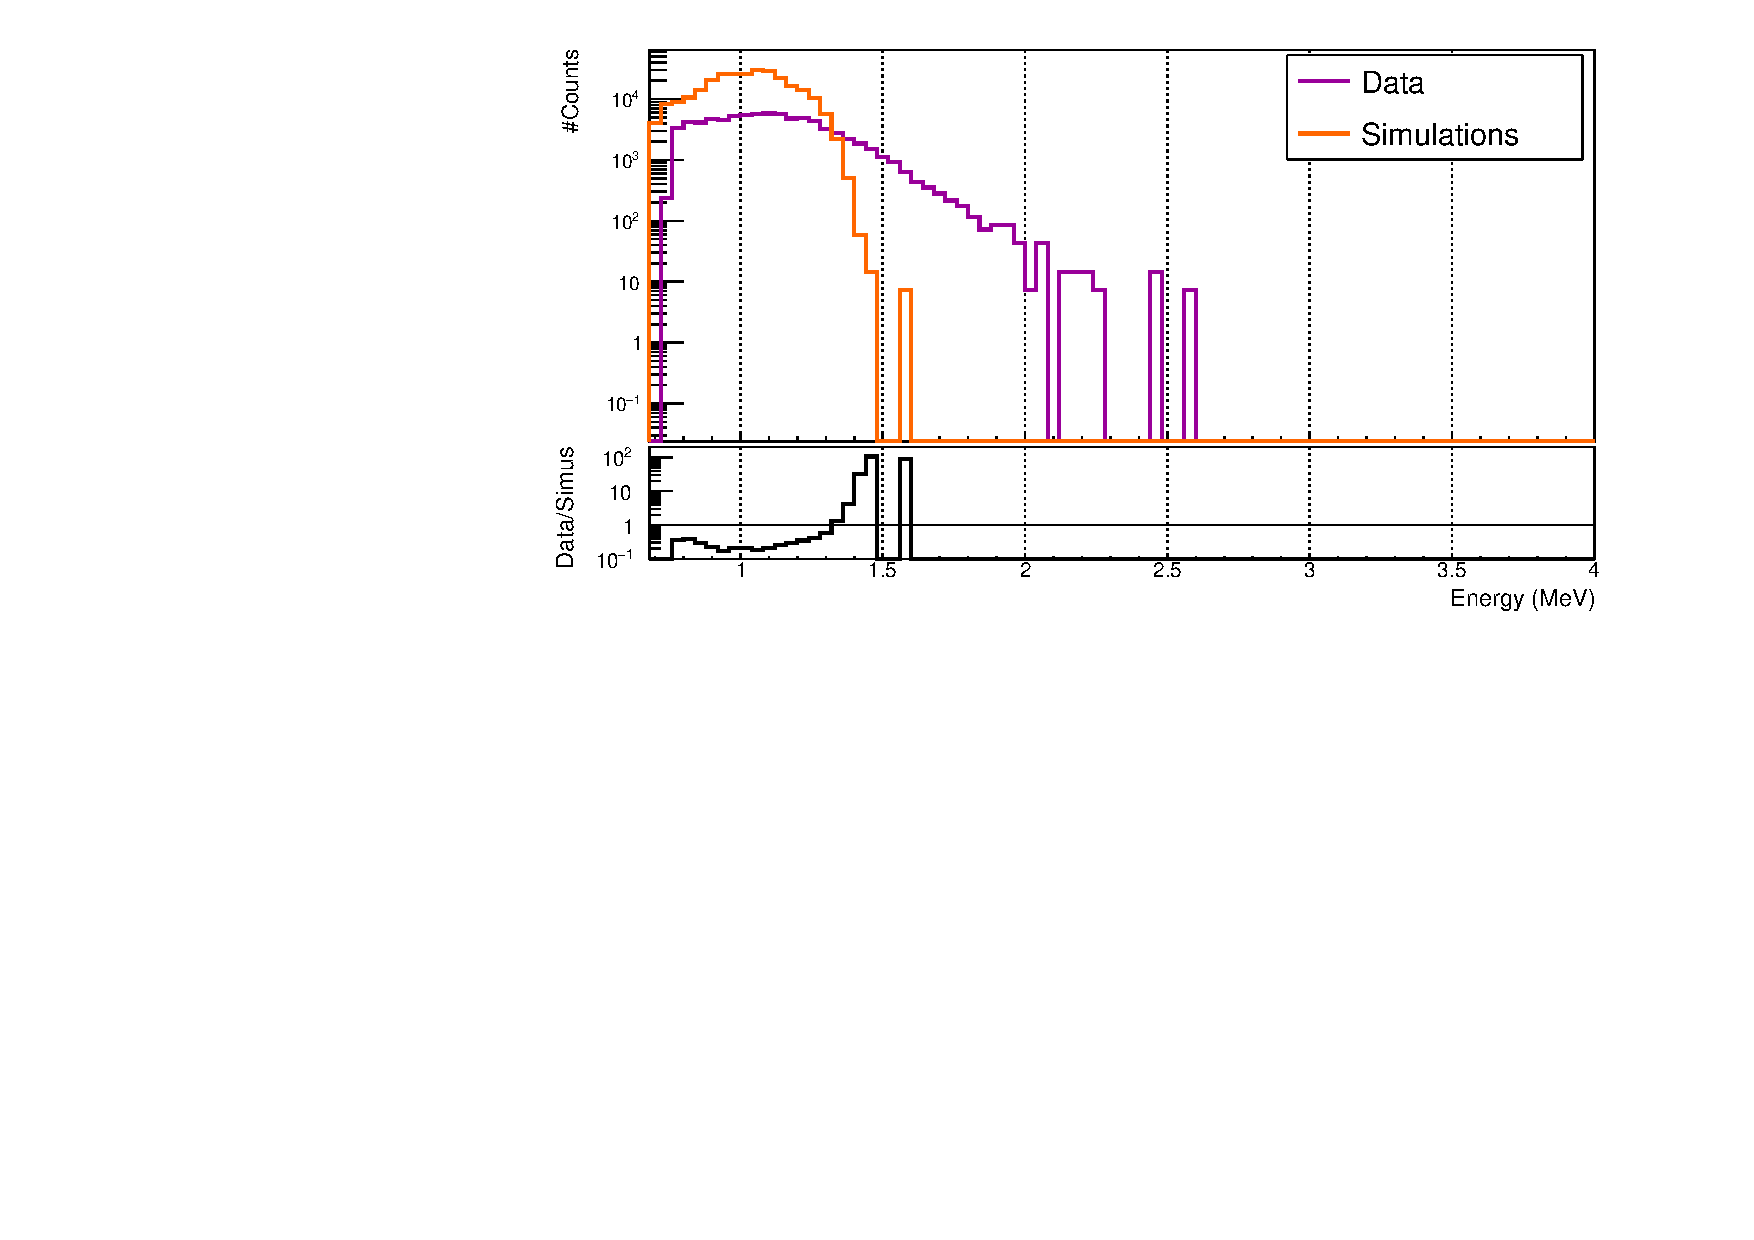
\includegraphics[width=17cm]{commissioning/fig_commissioning/Co_efficiency_detector.pdf}
%%   \caption{Top pad: energy spectra for simulated data (orange solid line) and real data (purple solid line) in logarithmic scale.
%%     Bottom pad: ratio of real data over simulated data for each bin in logarithmic scale.
%%     \label{fig:detector_efficiency}}
%% \end{figure}
%% The simulated data are normalised to the source activity and acquisition time.


%% Firstly, the energy resolution of the calorimeter blocks.
%% Secondly, at the time of the data taking, optical modules where not equalised in gain.
%% The real data energy spectrum is also characterised by a high energy part.
%% This may be due to external background events, which are not taken into account in the simulated data.
%% In Sec.~\ref{subsec:bkg_estimation} is presented a background analysis to investigate the high energy part of the energy spectrum, and better understand the data.


%% %% Given the amount of real and simulated events, we conclude that the detection efficiency is $29$\%.
%% %% Numerous parameters can affect the detection efficiency.
%% %% \begin{itemize}
%% %% \item Read out efficiency is mainly driven by
%% %% \end{itemize}



%% %% Efficiency is going to be improved.


%% * a finir *


%% The last step before going into detail in optical modules' timing resolution study is to determine the detector efficiency of the SuperNEMO demonstrator, during the Cobalt acquisition week.

\subsection{Determination of the individual timing resolution of each optical module}

%% Optical modules have been characterised before installation.
%% Performing simulations of \Co\ disintegration

\subsubsection*{Time difference distributions}

The final goal of this analysis is to determine the time resolution of optical modules, due to the scintillator time dispersion.
As displayed in Fig.~\ref{fig:Co_decay_scheme}, the two photons of Cobalt $60$ are emitted in coincidence compared with the time resolution expected for SuperNEMO.
The selections described in Sec.~\ref{subsec:Co_datacut} aim to maximise the signal to background ratio, the signal being the detection of two $\gamma$'s interacting in two different optical modules.

The two $\gamma$'s, travelling at speed of light in air, reach the two optical modules at two different times $t^{\gamma}_{i}$.
This time-of-flight is defined from the collected charge sampling at PM anode and received by the electronic readout (using the CFD method described in Chapter~\ref{ch:commissioning}).
These topologies are likely to happen for all combinations of pairs of optical modules.
Therefore, we can construct a $\Delta t^{\text{pair}}$ distribution for each pair of OM, defined as the time difference between two calorimeter hits $\Delta t^{\text{pair}} = t^{\gamma}_{A} - t^{\gamma}_{B}$.
Here, one of the two optical modules, namely the $A$, is chosen as reference.

In Fig.~\ref{fig:Co_deltat} is presented an example of a $\Delta t^{\text{pair}}$ distribution, for a given pair of optical modules, both for the simulated and real data, with the Cobalt source set in position $5$.
%% on ne regarde des coincidences que pour paires OM sur un même mur
\begin{figure}[h]
  \centering
  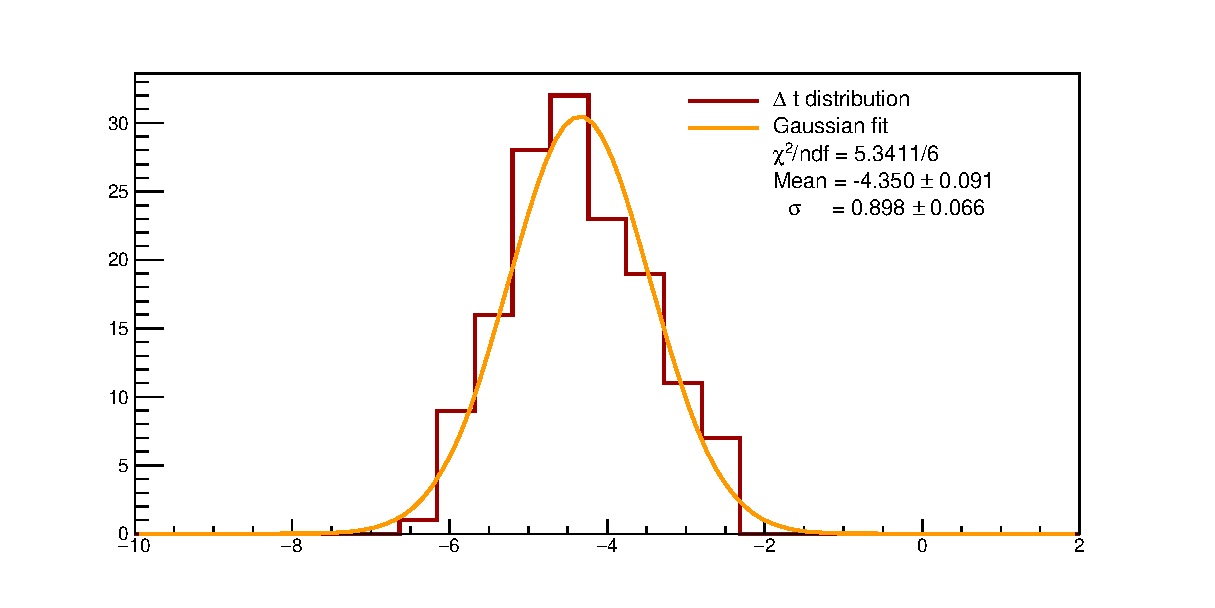
\includegraphics[width=15cm]{commissioning/fig_commissioning/Co_deltat_distrib_ex.eps}
  \caption{$\Delta t^{\text{pair}}$ distributions for real data (green solid line) and simulated data (dark red solid line).
    Two Gaussian fits (dotted line) are displayed and fit parameters are given in the legend box.
    The two distributions do not have the same mean because optical modules are not aligned in time.
    However, this does not disturb the time resolution measurements.
    \label{fig:Co_deltat}}
\end{figure}
The two distributions present different behaviours in terms of means and standard deviations.
This can be explained by two distinct reasons.

Firstly, as exposed in Sec.~\ref{subsec:OMtimeResponse}, in the framework of this study, the calorimeter part of the SuperNEMO demonstrator was considered as perfect in terms of time reconstruction, in the simulation processed.
All optical modules' time resolutions, whose main contributions are presented in Sec.~\ref{subsec:OMtimeResponse}, were set to $0$ ns.
We retrieve such a setting in the $\Delta t^{\text{pair}}$ distribution for simulated data.
As a consequence, the standard deviation, for this pair of optical module, is higher for real data than for simulated data.
Even though the case presented is just an example for a given pair of OM, we will see this is a general result for all pairs of optical modules.

Secondly, at this time, some differences remain between what is simulated and the real demonstrator performances.
In fact, as the demonstrator is in commissioning phase, some calorimeter detection characteristics are not yet included in the Falaise simulations, and affect the real data results (characterisation of optical modules' energy resolution, implementation of particle time-of-flight shifting due to coaxial cables...).
We observe such differences in the two distributions means: the data distribution is shifted by $3.7$ ns compared to the simulation distribution.
This result was expected: for the moment, the Falaise software does not take into account, in the reconstruction process, the time made by the electric signal to travel from a PM divider to the electronic readout, discussed in Sec.~\ref{sec:reflecto} of Chapter \ref{ch:commissioning}.
In other words, the time difference distribution for a given pair of optical module is affected by the difference of lengths of the two coaxial cables.
This is an important parameter directly affecting the mean time difference between two distinct optical modules detecting particles in coincidence.
Although simulations do not perfectly picture the full detector performances, real data and simulation can be compared, since we understand these differences.
Moreover, both the real and simulated data are affected by parameters such as the distance from the Cobalt source to the wall, or the distance between the two considered optical modules.

A $\Delta t^{\text{pair}}$ distribution exists for each pair of optical modules detecting two events in the time coincidence window.
The least square method is used to fit the distributions, which minimises the difference between the measured value and the fitted value.
A mean and a standard deviation is then defined for each pair of optical module whose fitted data has $\chi^{2}/\text{dof}<4$.
Therefore, each pair of optical module is characterised by the mean and standard deviation of its corresponding $\Delta t^{\text{pair}}$ distribution.
The standard deviation, noted as $\sigma_{t}^{\text{pair}}$ in the figure legend, corresponds to the uncertainty on time measurement for this peculiar pair of OM.
Therefore, a value of the time uncertainty $\sigma_{t}^{\text{pair}}$ can only be given for a proportion of total optical modules.

As the detector in commissioning phase, the acquisition was taken with $254$ optical modules\footnote{Three OMs are damaged on the French wall (*ref commissioning*) and three photomultipliers were not well aligned in gain at this time, and had to be removed from the analysis.}.
In this study, we only consider $8$ inches PMs, hence this analysis aims to characterise the time resolution of $214$ OMs, representing $22791$ different possible combinations of pairs.
In Fig.\ref{fig:Co_corr_sigma} are presented the $\sigma_{t}^{\text{pair}}$ values, both for simulated and real data.
\begin{figure}[h]
  \centering
  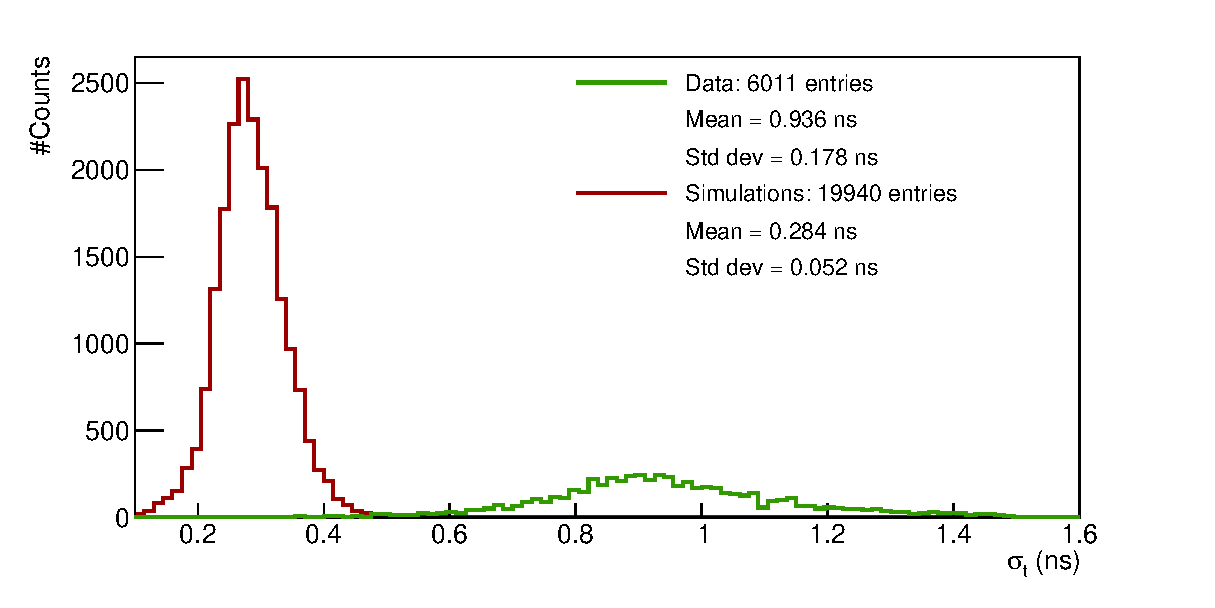
\includegraphics[width=15cm]{commissioning/fig_commissioning/Co_corr_sigma.eps}
  \caption{$\sigma_{t}^{\text{pair}}$ distribution for pairs of optical modules.
    \label{fig:Co_corr_sigma}}
\end{figure}
In the first place, we notice the mean $\sigma_{t}^{\text{pair}}$ value for simulations is lower than for real data.
As explained above, this difference is caused by the perfect calorimeter time resolution for simulations on one side, and by the detector characteristics not yet implemented in the simulation software on the other side.
This second statement is also behind the larger value of the real data distribution's standard deviation.
In fact, for the simulated case, $\Delta{t}$ distributions, of which an example is given in Fig.~\ref{fig:Co_deltat}, have comparable $\sigma_{t}^{\text{pair}}$ values, for all pairs of optical modules.
This is not the case for the real data: the $\sigma_{t}^{\text{pair}}$ value for a given pair of OM depends on the difference between the two coaxial cable lengths.
And this length difference being specific for each pair of optical module.

Moreover, we succeeded characterising $\sigma_{t}^{\text{pair}}$ values for $26$\% of pairs of optical blocks for real data, against $87$\% for simulations.
In fact, the more one optical module is from the source, the more it is background dominated.
As we explained, such a value is provided for a OM pair only if the fit of the corresponding $\Delta t^{\text{pair}}$ distribution is of high-quality.
Therefore, the optical modules for which the fit successes are the ones around the source.
This is not valid for simulations are we only have Cobalt events, and no background is simulated.

In Fig.\ref{fig:Co_sigma_distance} is displayed the number of characterised optical blocks, with the distance between the reference block and the Cobalt $60$ source, in units of block width.
\begin{figure}[h]
  \centering
  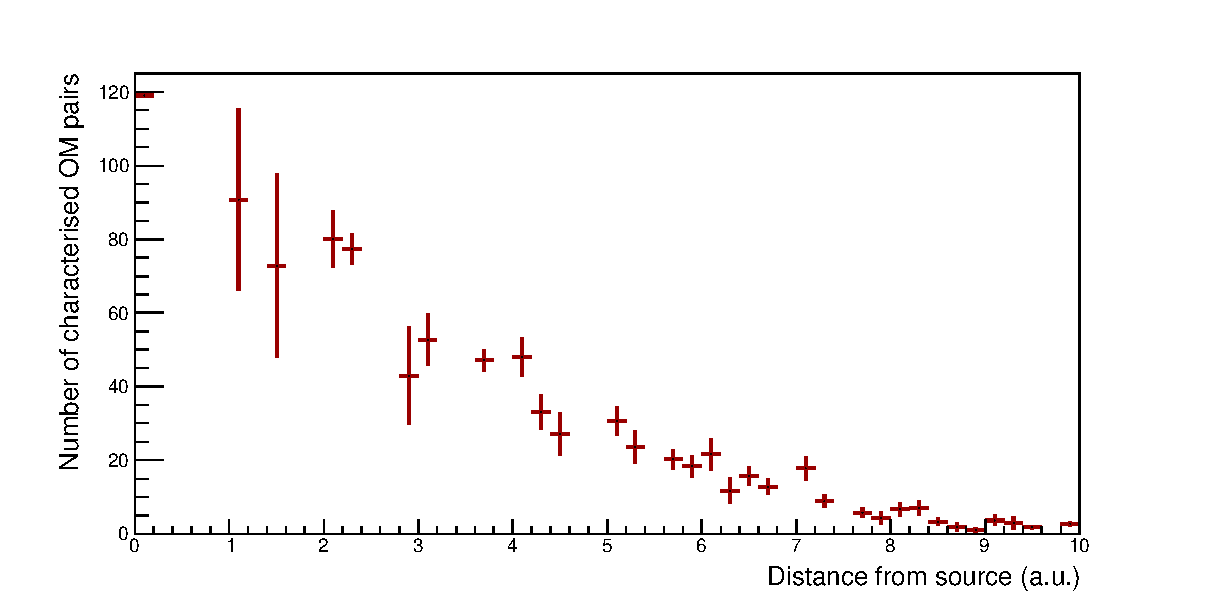
\includegraphics[width=15cm]{commissioning/fig_commissioning/Co_sigma_distance.eps}
  \caption{Number of characterised OM pairs, as a function of the distance between reference OM and source.
    \label{fig:Co_sigma_distance}}
\end{figure}
For a given distance from the source, the amount of characterised OM is lower for the real data case than for the simulated one.
This explains the different amount of characterised OMs for real and simulated data.

We presented results on the uncertainty on time measurement for pairs of optical module, $\sigma_{t}^{\text{pair}}$.
However, we are interesting in providing such values, independently for each optical modules.
Therefore, in the following, we present the algorithm we used to provide $\sigma_{t}^{\text{indep}}$ values.



%%fig distrib mean and sigma

\subsubsection*{Decoupling of $\sigma_{t}^{\text{pair}}$ values}

We have determined $\sigma_{t}^{\text{pair}}$ for some of the pairs of OMs on the French wall.
For example, if we take the source closest OM (OM located at the centre of the French main calorimeter wall), it has coincidence events with a certain number of other optical blocks.
Among them, $119$ different $\Delta t^{\text{pair}}$ distributions are fitted, therefore $119$ values of $\sigma_{t}^{\text{pair}}$ are stored.
And this work is done for each counting optical module taken as reference.
All following steps aim to determine the individual $\sigma_{t}^{\text{indep}}$.

We want to evaluate this value for the closest OM from the source, let us number it $0$.
We have access to the number of coincidence events this OM has with each other OMs.
We pick up the two OM that have the larger number of coincidence events with this reference OM, with their associated $\sigma_{t}^{\text{indep}}$ and mean energies.
We number them as $1$ and $2$.
Therefore, to find the value of $\sigma_{t}^{\text{indep}}$, we have to solve a set of $3$ linear equations:
\begin{align}
  (\sigma_{t}^{0,1})^{2} &= \frac{(\sigma_{t}^{0})^{2}}{\bar{E_{0}}} + \frac{(\sigma_{t}^{1})^{2}}{\bar{E_{1}}}\nonumber \\
  (\sigma_{t}^{0,2})^{2} &= \frac{(\sigma_{t}^{0})^{2}}{\bar{E_{0}}} + \frac{(\sigma_{t}^{2})^{2}}{\bar{E_{2}}}\\
  (\sigma_{t}^{1,2})^{2} &= \frac{(\sigma_{t}^{1})^{2}}{\bar{E_{1}}} + \frac{(\sigma_{t}^{2})^{2}}{\bar{E_{2}}} \nonumber\,,
  \label{eq:Co_sigma}
\end{align}
where $\sigma_{t}^{i}$ is the individual uncertainty on time measurement for the block $i$.
Solving simultaneously these equations comes down to diagonalise the matrix $S$ defined as
\begin{equation}
  S =
  \begin{pmatrix}
    1/\bar{E_{0}} & 1/\bar{E_{1}} & 0 \\
    1/\bar{E_{0}} & 0 & 1/\bar{E_{2}} \\
    0 & 1/\bar{E_{1}} & 1/\bar{E_{2}}
  \end{pmatrix}
  .
\end{equation}

We now generalise this method to all possible combinations of OM pairs for which we have informations on $\sigma_{t}^{\text{pair}}$.

\subsubsection*{Estimating the variance}



\subsection{Conclusion}
\begin{itemize}
\item il fauddrait au moins tenir compte du bdf qui est les decays de la source
\item il nous faut des simus bkg
\item il nous faut un run bkg
\item ça marche bien
\item il faudrait refaire une manip avec PMs alignés
  \item On aurait pu décorréler les sigmas en utilisant toutes les combinaisons possibles, mais il aurait fallu faire masse de simus pour déterminer les covariances
\end{itemize}


%%%%%%%%%%%%%%%%%%%%%%%%%%%%%%%%%%%%%%%%%%%%%%%%%%%%%%%%%%%%%%%%%%%%%%%%%%%%%%%%%%%%%%%%%%%%%%%%%%%%%%%%%%%%%%%%%%%%%%%%%%%%%%%%
\section{The Light Injection System}
\label{sec:LIS}



\subsection{Light injection system commissioning}


In the LI system design, the SuperNEMO demonstrator has been segmented in $10$ areas.
Each area receives light from one given LED

Primary/secondary
Each LED lights
Group LEDs/area



\subsection{Time resolution of optical modules}



%% \begin{figure}[h]
%%   \centering
%%   \includegraphics[width=10cm]{commissioning/fig_commissioning/}
%%   \caption{
%% \label{fig:}}
%% \end{figure}



%% \begin{figure}[h]
%% \centering
%% \begin{subfigure}[t]{0.48\textwidth}
%%   \centering
%%   \includegraphics[width=1.1\textwidth]{commissioning/fig_commissioning/}
%%   \captionsetup{justification=centering}
%%   \caption{
%%     \label{subfig:}}
%% \end{subfigure}
%% \hfill
%% \begin{subfigure}[t]{0.48\textwidth}
%%   \centering
%%   \includegraphics[width=1.1\textwidth]{commissioning/fig_commissioning/}
%%   \captionsetup{justification=centering}
%%   \caption{
%%     \label{subfig:}}
%% \end{subfigure}
%% \caption{
%%   \label{fig:}}
%% \end{figure}
